%! TeX program = lualatex
%---------------------------ALLGEMEINE IMPORTS-------------------------------------
\documentclass[12pt,english,ngerman]{scrartcl}
\input{./protokoll_template/template.latex/input/shared_preamble.tex}

% Kopfzeile
\ihead{WS22\\
	16.12.2022} \chead{\textsc{Stark} Matthias - 12004907 \\
	\textsc{Philipp} Maximilian - 11839611}
\ohead{FLAB 1 \\
	Spektrograph}
% Fußzeile

\begin{document}

\section{Aufgabenstellung\label{sec:Aufgabenstellung}}

\begin{itemize}
	\item Adjustierung des Prismenspektrographen, der Linsen und der Prismen im
	      Spektrographen, um ein Spektrum für alle Lichtquellen abzubilden.
	\item Aufnahme des Spektrums von den Verschiedenen Lichtquellen und der Probe.
	\item Aufnahme der Spektren der gleichen Lichtquellen mit dem Gitterspektrographen.
	\item Erzeugung der Dispersionskurve des Prismenspektrographen.
	\item Bestimmung des Auflösevermögen der beiden Spektrographen.
	\item Bestimmung der Wellenlänge der Jod-Absorbtionsbandkanten.
	\item Bestimmung der Dissoziationsenergie des Jodmoleküls.
\end{itemize}

\section{Grundlagen}\label{sec:Grund}

\subsection{Molekulare Spektroskopie}

Wenn elektromagnetische Strahlung mit einem Molekül in Wechselwirkung tritt,
kann sie absorbiert, emittiert oder gestreut werden, je nach der Energie der
Strahlung und den Energieniveaus des Moleküls. Die Energie der Strahlung wird
durch ihre Wellenlänge oder Frequenz bestimmt, und die Energieniveaus des
Moleküls werden durch seine elektronische Struktur, seine Vibrations- und
Rotationsmoden bestimmt.

Die Absorption oder Emission elektromagnetischer Strahlung durch ein Molekül
kann als Änderung der Intensität der Strahlung beim Durchgang durch die Probe
beobachtet werden. Diese Änderung kann mit einem Spektrometer gemessen und zur
Untersuchung der elektronischen Struktur und Bindung des Moleküls sowie seiner
Schwingungs- und Rotationsenergieniveaus verwendet werden.

\subsection{Prismenspektrograph}
Ein Prismenspektrograph ist ein Spektrograph, der ein Prisma verwendet, um die
elektromagnetische Strahlung in ihre einzelnen Wellenlängen oder Frequenzen zu
zerlegen. Er besteht aus einer Lichtquelle, einem Prisma und einem Detektor und
wird verwendet, um das elektromagnetische Spektrum einer Probe grafisch
darzustellen.

Die Lichtquelle eines Prismenspektrographen ist in der Regel eine Lampe oder
ein Laser, mit dem die Probe beleuchtet wird. Die Probe wird in den
Strahlengang gestellt, und ein Teil der elektromagnetischen Strahlung wird von
der Probe absorbiert, emittiert oder gestreut.

Das Prisma ist ein transparentes optisches Element, das aus einem brechenden
Material wie Glas oder Quarz besteht. Es wird in den Weg der
elektromagnetischen Strahlung gestellt und dient dazu, die Strahlung in ihre
einzelnen Wellenlängen oder Frequenzen zu zerlegen. Das Prisma funktioniert,
indem es die Strahlung je nach Wellenlänge oder Frequenz in unterschiedlichen
Winkeln bricht. Dies führt dazu, dass sich die verschiedenen Wellenlängen oder
Frequenzen der Strahlung nach dem Snelliuschen Brechungsgesetz,
\autoref{eq:snel}, ausbreiten und ein Spektrum bilden. 

\begin{equation}
	\frac{\sin{\theta_1}}{\sin{\theta_2}} = \frac{n_1(\lambda)}{n_2(\lambda)}
	\label{eq:snel}
\end{equation}

$\theta_1$ und $\theta_2$ bezeichnet dabei den Eintritts bzw. Austrittswinkel und $n_1$ und $n_2$ die entsprechenden Brechzahlen.
Der Strahlengang durch ein Prisma ist in folgender \autoref{fig:skizze} skizziert.

%todo cite

\begin{figure}[H]
	\begin{center}
		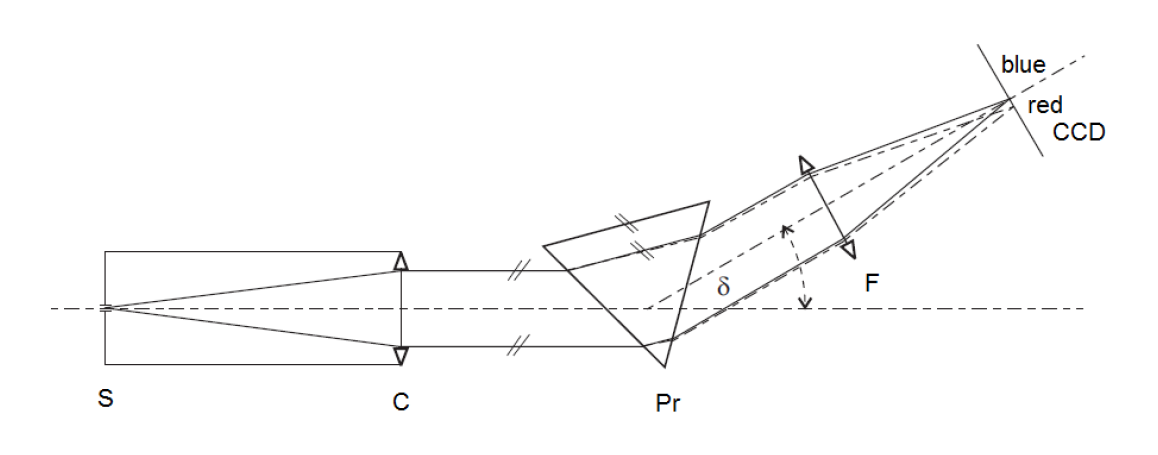
\includegraphics[width =\textwidth]{./figures/skizze.png}
	\end{center}
	\caption[Skizzierter Strahlengang durch ein Prisma] {Skizzierter Strahlengang durch ein
		Prisma, entnommen aus \cite{unterlagen} \\
		S \(\dots\) Spalt                       \\
		C \(\dots\) Kondensor-Linse             \\
		Pr \(\dots\) Prisma                     \\
		F \(\dots\) Fokusier-Linse              \\
		CCD \(\dots\) Schirm                    \\
		$\delta$ \(\dots\) Brechungswinkel
	}\label{fig:skizze}
\end{figure}

Der Detektor eines Prismenspektrographen ist in der Regel eine Kamera oder ein
Aufzeichnungsgerät, mit dem die Intensität der elektromagnetischen Strahlung
über einen Bereich von Wellenlängen oder Frequenzen gemessen wird. Der Detektor
erzeugt ein Diagramm der Intensität der Strahlung in Abhängigkeit von der
Wellenlänge oder Frequenz, das als Spektrum bezeichnet wird.

\subsection{Gitterspektrograf}

Ein Echelle-Spektrograf ist ein Spektrograf, der ein Beugungsgitter, das so
genannte Echelle-Gitter, verwendet, um die elektromagnetische Strahlung in ihre
einzelnen Wellenlängen oder Frequenzen zu zerlegen. Er besteht aus einer
Lichtquelle, einem Echelle-Gitter, einem Kollimator, einer Kamera oder einem
Aufzeichnungsgerät und einer Brennebene.

Bei der Lichtquelle eines Echelle-Spektrographen handelt es sich in der Regel
um eine Lampe oder einen Laser, mit dem die Probe beleuchtet wird. Die Probe
wird in den Strahlengang gestellt, und ein Teil der elektromagnetischen
Strahlung wird von der Probe absorbiert, emittiert oder gestreut.

Das Echelle-Gitter ist ein Beugungsgitter, das aus einem transparenten
optischen Element wie Glas oder Quarz besteht und mit einem periodischen Muster
aus parallelen Linien versehen ist. Es wird im Strahlengang der
elektromagnetischen Strahlung angebracht und dient dazu, die Strahlung in ihre
einzelnen Wellenlängen oder Frequenzen zu zerlegen. Das Echelle-Gitter
funktioniert, indem es die Strahlung je nach ihrer Wellenlänge oder Frequenz in
unterschiedlichen Winkeln, nach \autoref{eq:beugung}, beugt. Dies führt dazu,
dass sich die verschiedenen Wellenlängen oder Frequenzen der Strahlung
ausbreiten und ein Spektrum bilden.

\begin{equation}
	d \sin{\theta} = n \lambda
	\label{eq:beugung}
\end{equation}

$d$ bezeichnet dabei den Gitterabstand, $\theta$ den Beugungswinkel, $n$ die entsprechende Ordnung und $\lambda$ die Wellenlänge.
Eine schematische Skizze des Strahlengangs ist in \autoref{fig:gitter} sichtbar.

\begin{figure}[H]
	\begin{center}
		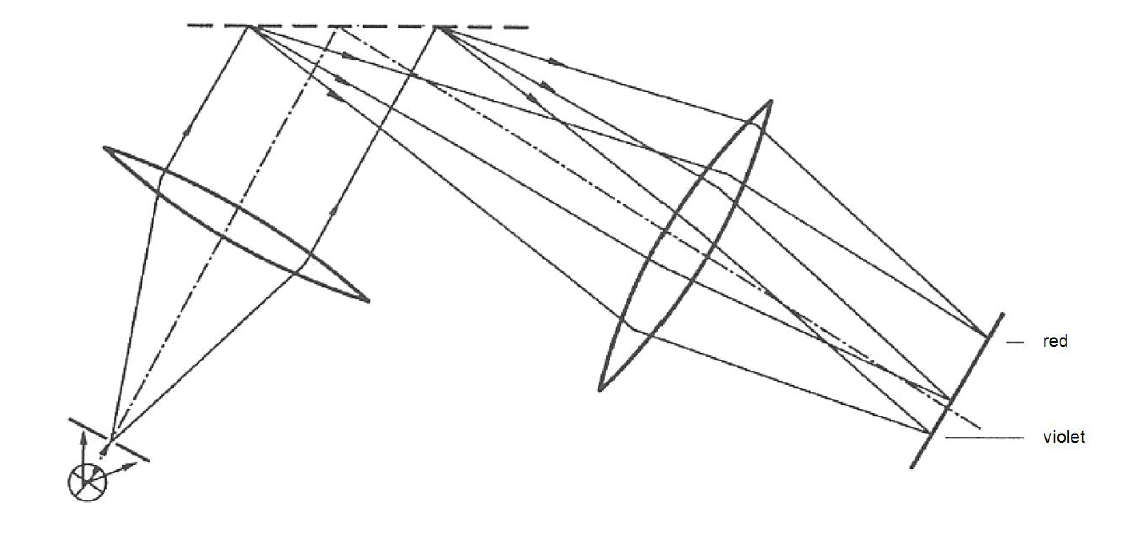
\includegraphics[width =\textwidth]{./figures/skizze_gitter.png}
	\end{center}
	\caption[Skizzierter Strahlengang durch ein Gitter] {Skizzierter Strahlengang durch ein
		Gitter, entnommen aus~\cite{unterlagen}
	}\label{fig:gitter}
\end{figure}

Der Kollimator ist eine Linse oder ein Spiegel, der dazu dient, die
elektromagnetische Strahlung zu kollimieren, d.h. zu einem parallelen Strahl zu
bündeln. Der Kollimator befindet sich hinter dem Echelle-Gitter und sorgt
dafür, dass die Strahlung auf die Kamera oder den Rekorder fokussiert wird.

Mit der Kamera oder dem Rekorder wird die Intensität der elektromagnetischen
Strahlung über einen Bereich von Wellenlängen oder Frequenzen gemessen. Es wird
ein Diagramm der Strahlungsintensität in Abhängigkeit von der Wellenlänge oder
Frequenz erstellt, das als Spektrum bezeichnet wird.

Die Brennebene ist die Ebene, in der das Spektrum gebildet wird, und sie
befindet sich in der Regel im Brennpunkt des Kollimators. Die Kamera oder der
Rekorder wird in der Fokusebene platziert, um die Intensität der
elektromagnetischen Strahlung zu messen.

%todo max brachst du noch irgendwelche formeln?
% Ja bitte noch allgemeine aufloesungs formel Extinktion dispersionsrelation, photoeffekt energie, wellenzahl zu wellenlangen relation

\section{Versuchsaufbau}\label{sec:aufbau}

\subsection{Prismenspektrograph}

Der Versuchsaufbau ist in folgender \autoref{fig:aufbau_Spektograph}
ersichtlich. Dabei wird die Position der Lichtquelle mit einem leeren
Linsenhalter auf der optischen Bank markiert, um später beim Wechsel der
Lichtquelle die selbe Position zu ermöglichen. Bei den Linsen wir dabei
versucht, den vorliegenden Lichtstrahl, so gut wie möglich, auf den
Eingangsspalt des Spektrographen zu fokusieren, um eine möglichst hohe
Intensität zu gewährleisten. Auch die Position, auf die die Iodzelle gestellt
wird, wird mit einem leeren Linsenhalter markiert.

\begin{figure}[H]
	\begin{center}
		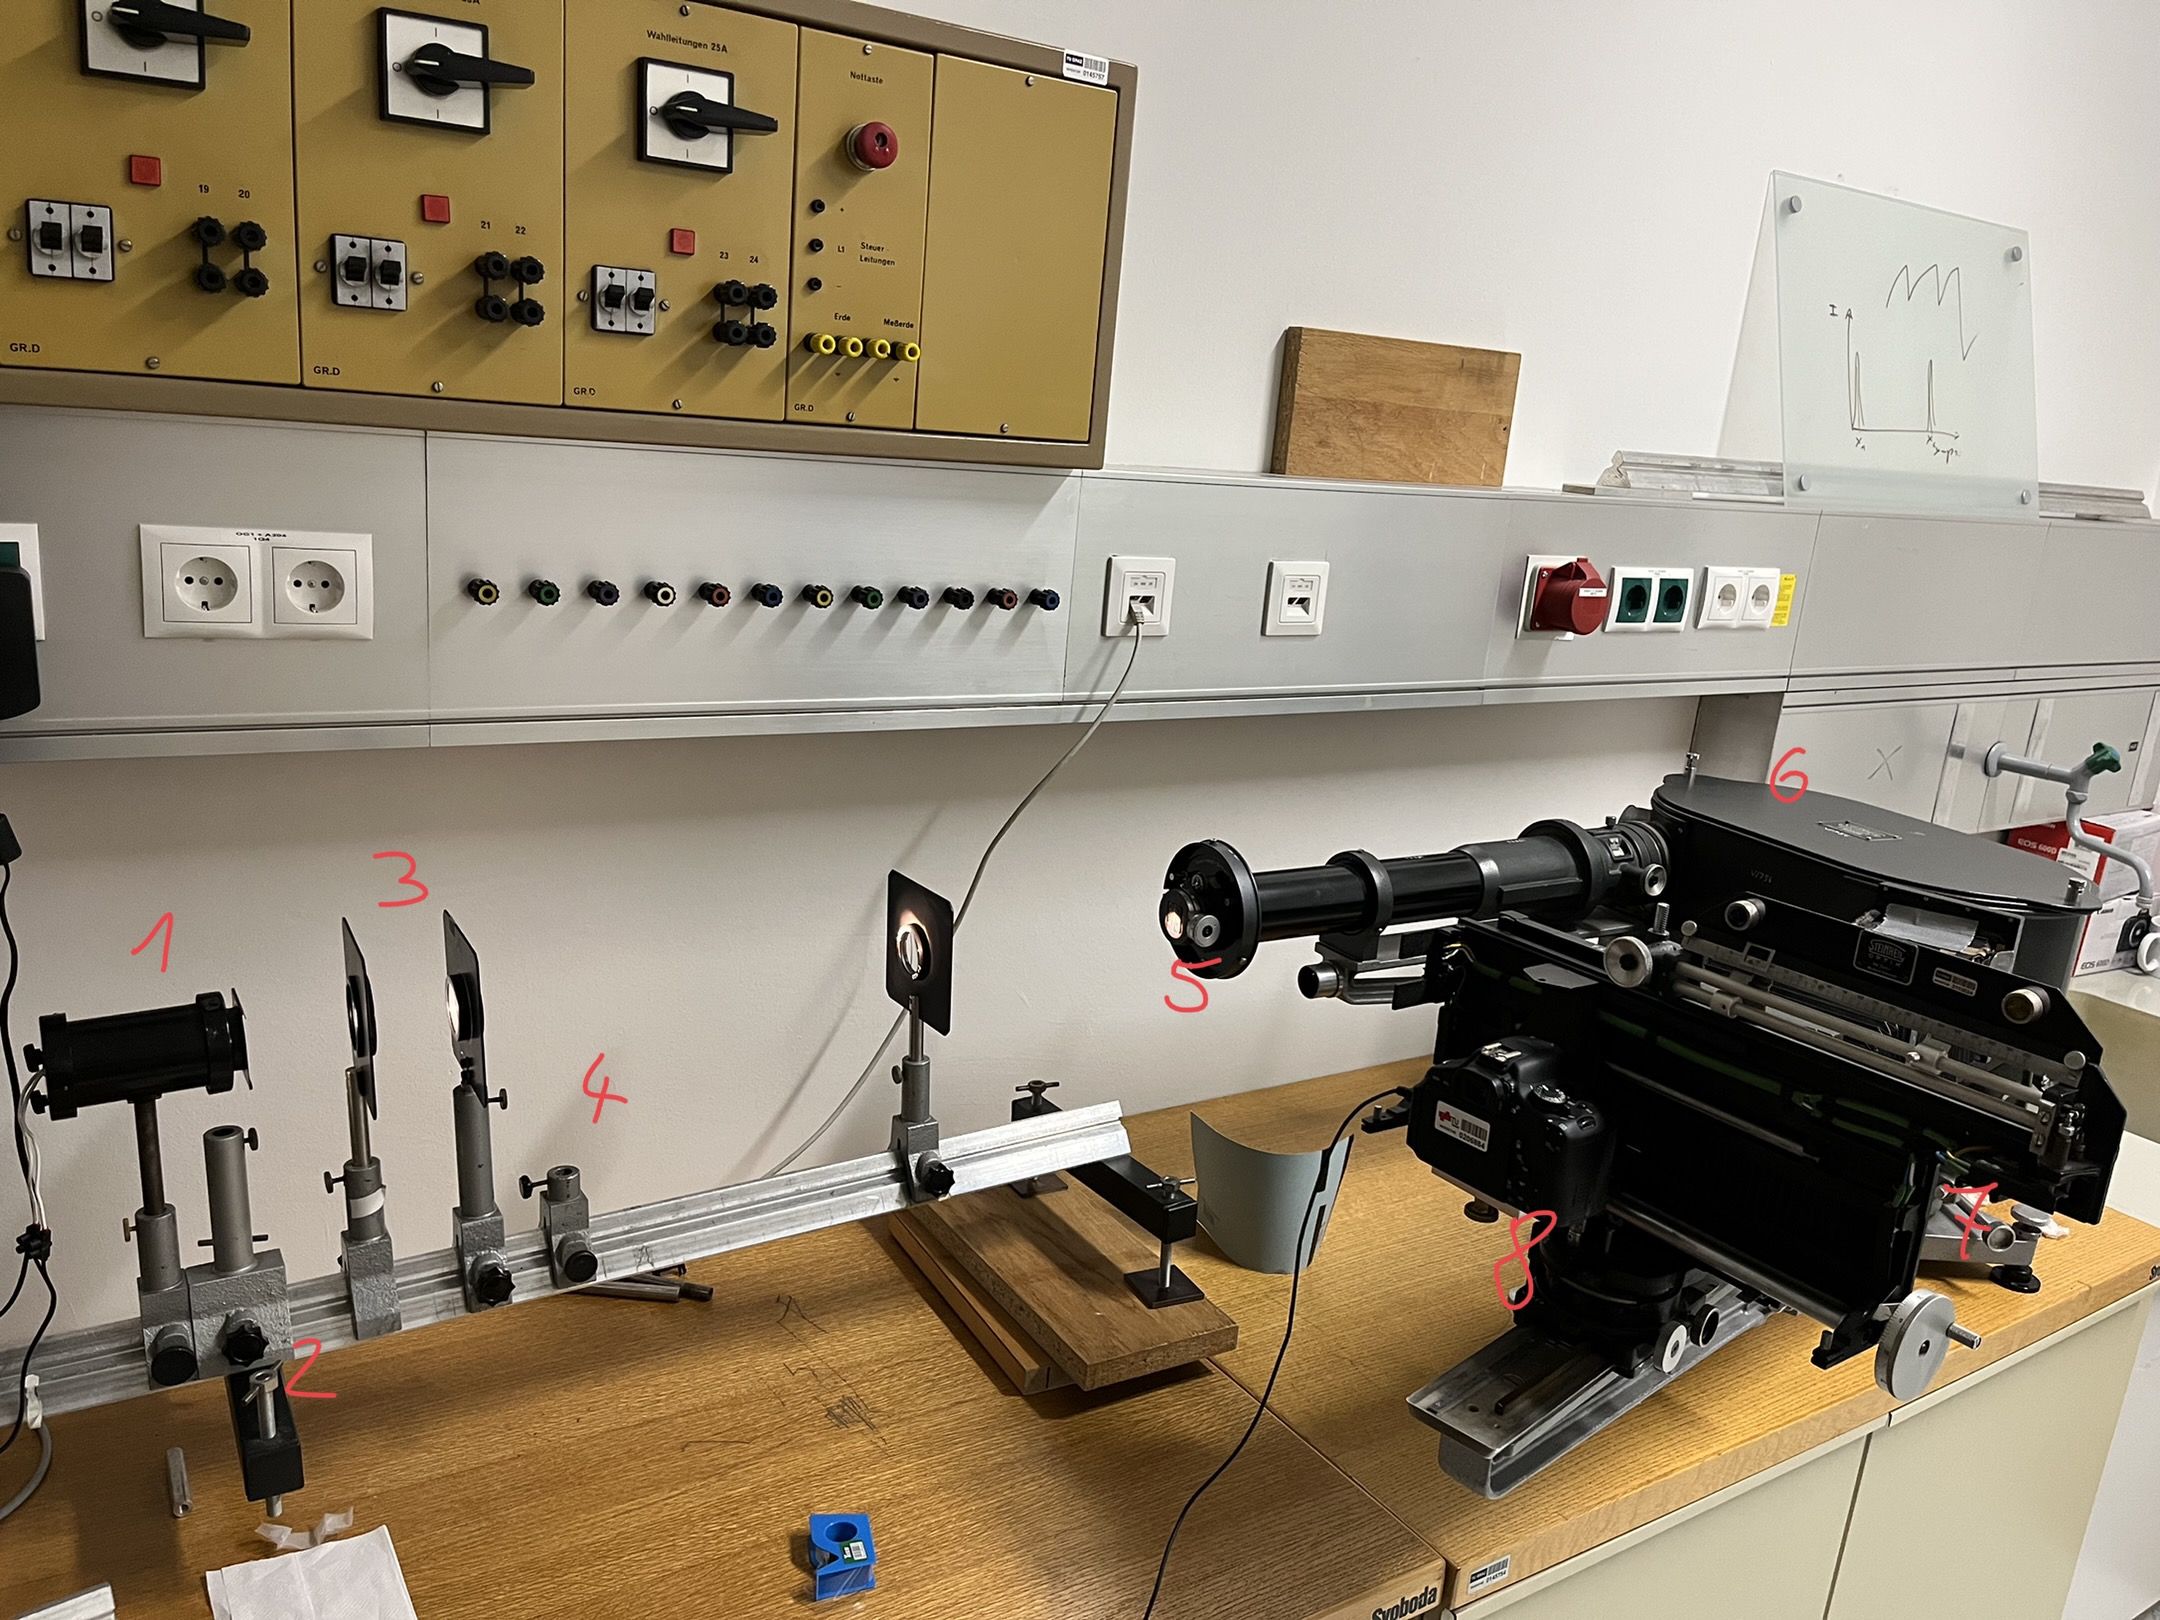
\includegraphics[width =\textwidth]{./figures/Spektograph.png}
	\end{center}
	\caption[Versuchsaufbau des Prismenspektrographen] {Versuchsaufbau des
		Prismenspektrographen                                                    \\
		1 \(\dots\) Lichtquelle                                                  \\
		2 \(\dots\) Markierung für die Lichtquelle                               \\
		3 \(\dots\) Verwendete Sammellinsen (Brennweiten: v.l.n.r. 250, 50, 120) \\
		4 \(\dots\) Markierung für die Iodquelle                                 \\
		5 \(\dots\) Eintrittsspalt in den Spektrographen                         \\
		6 \(\dots\) Prismen in Spektrographen                                    \\
		7 \(\dots\) Halterung für Kamera                                         \\
		8 \(\dots\) Befestigte Kamera
	}\label{fig:aufbau_Spektograph}
\end{figure}

Im inneren des Spektrographen müssen nun die Prismen durch vorsichtiges
Verdrehen richtig eingestellt werden, sodass der eintreffende Lichtstraht durch
die 3 Prismen zur Ausgangsöffnung abgelenkt wird und dort das komplette
Spektrum, innerhalb des Schirms sichtbar ist. Um dies gut beurteilen zu können,
wird ein Streifen Klebeband über die entsprehende Öffnung geklebt, sodass das
gebrochene Licht gut sichtbar wird. Die entsprechenden Positionen der Prismen
sind in \autoref{fig:prismen} sichtbar.

\begin{figure}[H]
	\begin{center}
		\includegraphics[width =0.5\textwidth]{./figures/Prismen.png}
	\end{center}
	\caption[Anordnung der Prismen im Spektrographen] {Anordnung der Prismen im
		Spektrographen
	}\label{fig:prismen}
\end{figure}

\subsection{Gitterspektograph}

Der Aufbau des Gitterspektrographen ist in \autoref{fig:aufbau_gitter}
sichtbar. Dabei wird der Sensor des Gitterspektrographen mithilfe einer
passenden Halterung direkt vor die Lichtquelle gestellt.
\begin{figure}[H]
	\begin{center}
		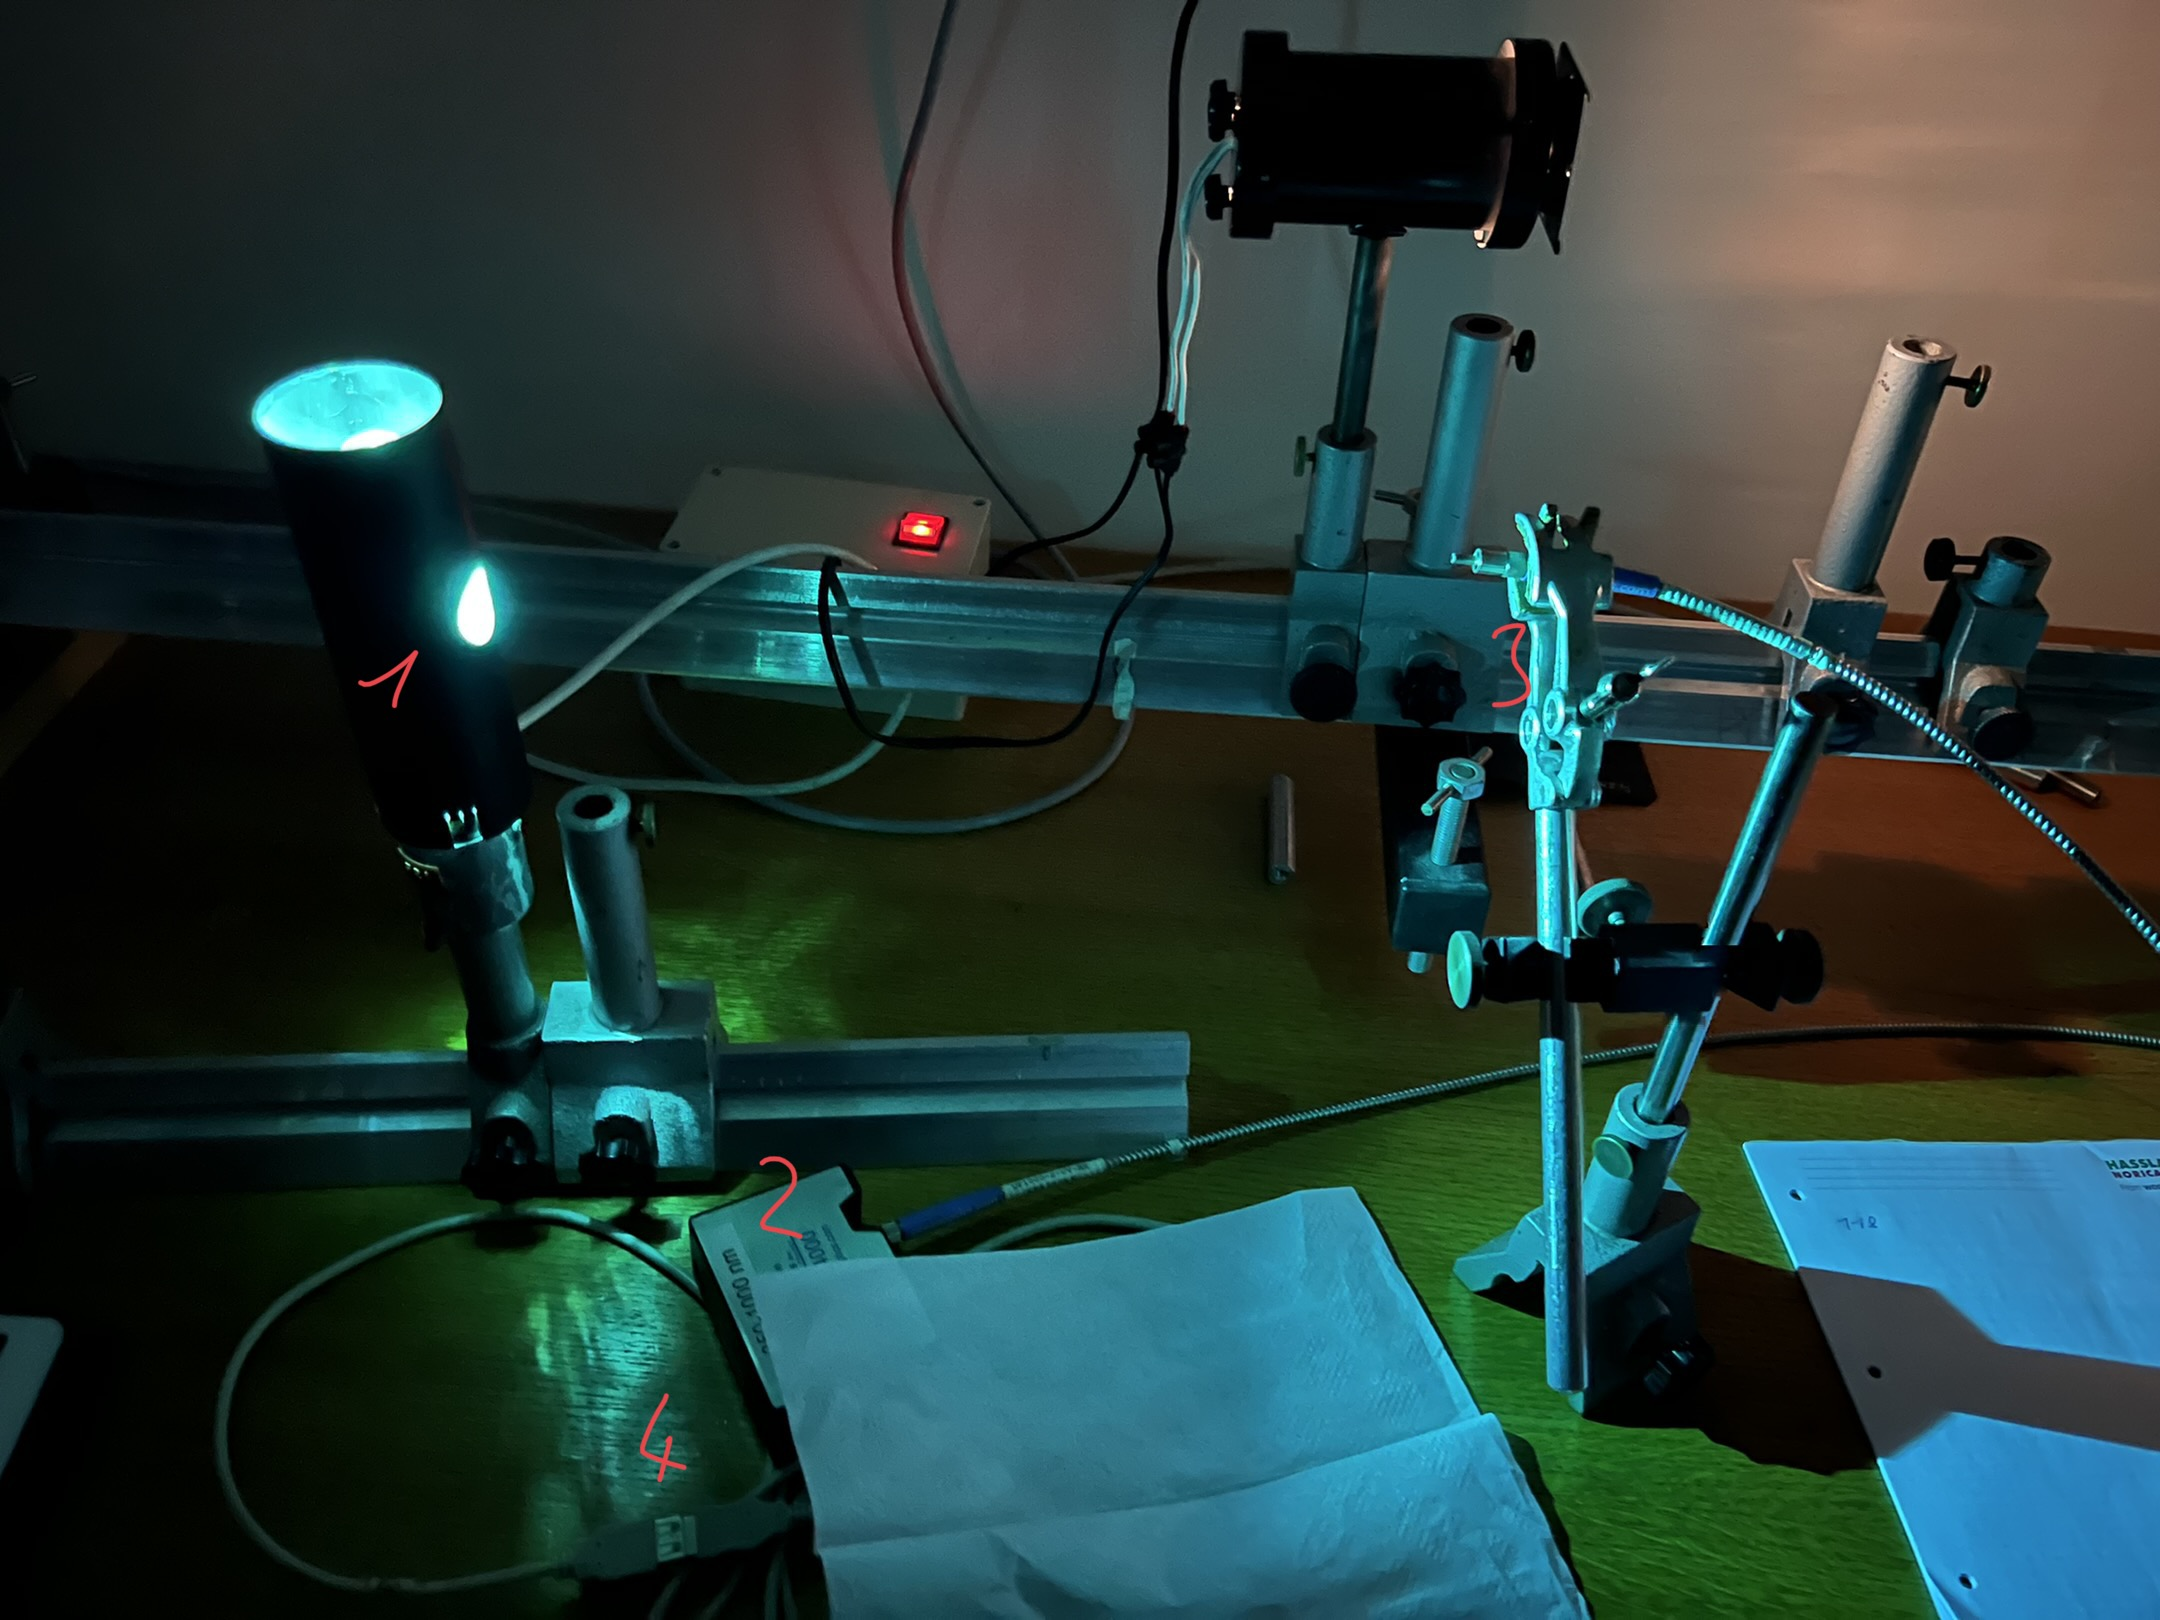
\includegraphics[width =\textwidth]{./figures/Gitterspektograph.png}
	\end{center}
	\caption[Versuchsaufbau des Gitterspektrographen] {Versuchsaufbau des
		Gitterspektrographen                  \\
		1 \(\dots\) Lichtquelle               \\
		2 \(\dots\) Gitterspektograph         \\
		3 \(\dots\) Sensor der Spektrographen \\
		4 \(\dots\) Schnittstelle für Computer
	}\label{fig:aufbau_gitter}
\end{figure}

\section{Geräteliste}\label{sec:geraeteliste}

Für den Versuch werden die in \autoref{tab:gerate} aufgelisteten Geräte
verwendet.

\begin{table}[H]
	\caption{Verwendete Geräte
	}
	\begin{tblr}{cells={font=\footnotesize}, colspec={lllll}}
		\textbf{Gerätetyp} & \textbf{Hersteller} & \textbf{Typ}     & \textbf{Inventar-Nr} & \textbf{Anmerkung} \\ 
		\toprule
		Prismaspektogaph   & Steinheil           &                  & 0153624              &                    \\ 
		Gitterspektograph  & Ocean Optics        & USB4000          & 0101417              & 350-1000 nm        \\ 
		Kamera             & Canon               & EOS 600D         & 0206884              & ohne Linse         \\ 
		Lichtleiter        & Ocean Optics        & OP1000-2-UV-BX   &                      &                    \\ 
		Hg-Dampflampe      &                     & Hg-Cd            & F21                  &                    \\ 
		Halogenlampe       & Leybold             &                  & F4                   &                    \\ 
		Iodprobe           & Spindler \& Hoyer   &                  & V / 154d             &                    \\ 
		Sammellinsen       &                     & f = 250, 50, 120 &                      & 3 x                \\ 
		Optische Bank      &                     &                  &                      & höhenverstellbar   \\ 
		Linsenhalter       &                     &                  &                      &                    \\ 
	\end{tblr}\label{tab:gerate}
\end{table}

%V/1003, Qu, V/748/4

\section{Durchführung und Messergebnisse}\label{sec:durchfuhrung}

\subsection{Prismenspektrograph}

Nachdem die Linsen und Prismen wie bereits in \autoref{sec:aufbau} angeführt,
aufgebaut wurden, wird das, von der Kamera erfasste, Spektrum am Computer mit
der Software SpectraSuite betrachtet. Es ist dafür zu sorgen, dass die
einzelnen Linien der Lichtquelle scharf erscheinen und eine möglichst gute
Nutzung der gesamten Breite des zur Verfügung stehenden Schirms vorliegt. Dies
wird durch Verstellen und anschließender Feinjustierung der Neigung und des
Abstands der Kamera zum Spektographen erreicht. Um das abgebildete Spektrum
sichtbar zu machen, wird ein Streifen Klebeband an der entsprechenden Stelle
des Spektrographen angebracht. Um dafür zu sorgen, dass kein Störlicht auf die
Kamera gelangt, wird das gesamte Raumlicht abgedunkelt und ein Karton seitlich
an die Kamera gehalten, um kein Licht seitlich von der Lichtquelle zu bekommen.

Weil nicht das gesamte Spektrum mit einem Foto aufgezeichnet werden kann wird
zunächst bestimmt, wie groß der erfasste Bereich ist. Dazu wird zunächst die
Kamera mithilfe der entsprechenden Kurbel so lange bewegt, bis der rote Peak
gerade am rechten Rand des Bildschirms verschwindet. Nun wird die Kamera, unter
Bestimmung der entsprechenden Distanz, solange weiterbewegt, bis sich diese
rote Linie am linken Rand des Bildschirms befindet. Dadurch wird die Distanz
des aufgezeichneten Spektrums bestimmt. Nun wird auf diese Art das gesamte
Spektrum aufgezeichnet, welches schließlich Bild für Bild zusammengesetzt
werden kann. Dabei ist zu beachten, dass das Spektrum immer von beiden
Lichtquellen und der Iodprobe festgehalten wird, bevor die Kameraposition
verschoben wird. Weil bei den verschiedenen Farbeindrücken unterschiedliche
Helligkeiten vorliegen, muss auch immer der Kontrast neu eingestellt werden.
Ein Bild eines Teils des Spektrums in entsprechenden Computerprogramm ist
symbolisch in folgender \autoref{fig:comp} sichtbar.

\begin{figure}
	\begin{center}
		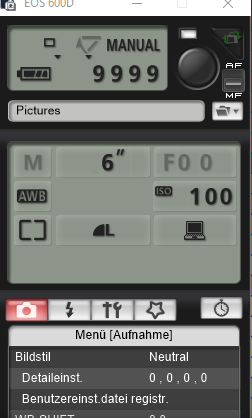
\includegraphics[width=0.15\textwidth]{figures/camerasoftware.png}
	\end{center}
	\caption{Das Software Interface für die Kontrolle der Kamera
	}\label{fig:comp}
\end{figure}

Um den Versuch repoduzieren zu können, sollte exakt der gleiche Spektrograph
verwendet werden. Alle abgelesenen und eingestellten Werte sind in folgender
\autoref{tab:einstellungen} ersichtlich. Weil die Messwerte nicht immer klar
von der entsprechenden Skala ablesbar waren wurde dies bei den Unsicherheiten
berücksichtigt und in der Tabelle in der entsprechenden Spalte vermerkt.

\begin{table}[H]
	\caption[Abgelesene Einstellungen]{Abgelesene Einstellungen                              \\
		$f_i \dots$ Brennweite der i-ten Sammellinse in mm    \\
		$f_k \dots$ Brennweite des Kollimators                \\
		$SP \dots$ Spaltbreite des Eingangsspalt              \\
		$x \dots$ Entfernung der Kamera                       \\
		$N_{Pi} \dots$ Neigung des i-ten Prismas (nicht in °) \\
		$N_{PT} \dots$ Neigung des Tisches in °               \\
		$N_{PK} \dots$ Neigung der Kamera in °
	}
	\begin{tabular}{|l|l|l|}
		\hline
		\textbf{Bezeichnung} & \textbf{Messwert}       & \textbf{Anmerkung zur Unsicherheit} \\ \hline
		$f_1$                & \SI{250}{\mm}           & Implizit gegeben                    \\ \hline
		$f_2$                & \SI{50}{\mm}            & Implizit gegeben                    \\ \hline
		$f_3$                & \SI{120}{\mm}           & Implizit gegeben                    \\ \hline
		$f_k$                & \SI{141.6(1)}{\micro\m} & Skala                               \\ \hline
		$SP$                 & \SI{80(1)}{\micro\m}    & Mikrometerschraube                  \\ \hline
		$x$                  & \SI{43.2(1)}{\mm}       & Skala                               \\ \hline
		$N_{P1}$             & \SI{65(2)}{}            & Geschätzt mit Entfernungsmessung    \\ \hline
		$N_{P2}$             & \SI{10.5(5)}{}          & Abgelesen auf entsprechender Skala  \\ \hline
		$N_{P3}$             & \SI{6.5(2)}{}           & Abgelesen auf entsprechender Skala  \\ \hline
		$N_{PT}$             & \SI{10.88(2)}{\degree}  & Skala                               \\ \hline
		$N_{PK}$             & \SI{20(5)}{\degree}     & Augenmaß                            \\ \hline
	\end{tabular}\label{tab:einstellungen}
\end{table}

\subsection{Gitterspektograph}

Um das Spektrum mithilfe des Gitterspektrographen zu analysieren, wird der
Aufbau aus \autoref{sec:aufbau} in den Strahlengang der entsprechenden Probe
gestellt. Der Computer wird über die entsprechende Verbindung angeschlossen und
das Auswertungsprogramm gestartet. Bei der genauen Position des Sensors wird
dabei darauf geachtet, dass die verzeichneten Peaks möglichst groß werden,
diese aber nicht saturieren. Ein Ausschnitt dieser Einstellungen im Programm
ist dabei symbolisch in \autoref{fig:comp_gitter} sichtbar.

\begin{figure}[H]
	\begin{center}
		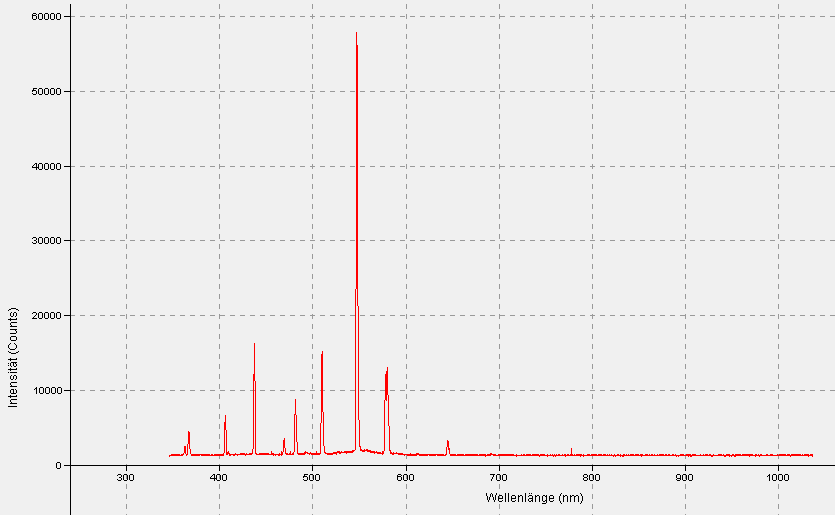
\includegraphics[width=0.95\textwidth, height=4cm]{figures/gitterSpektComp.png}
	\end{center}
	\caption{Aufnahme des Referenzspektrums mittels des Gitterspektrographs und Software
	}\label{fig:comp_gitter}
\end{figure}

\section{Auswertung}\label{sec:auswertung}

Um zu sehen wie sich die Unsicherheit der Messungen bis in die Ergebnisse
fortpflanzt, ist erweiterte Gauss-Methode verwendet worden. Die Grundlagen
dieser Methode stammen von den Powerpointfolien von
GUM~\cite{wolfgang_kessel_isobipm-gum_2004}. Für die Auswertung ist die
Progammiersprache Python im speziellen die Pakete \verb#labtool-ex2#,
\verb#pandas#, \verb#sympy#, \verb#lmfit# zur Hilfe genommen worden.
\verb#lmfit# wurde für das Fitten hergenommen, \verb#sympy# wurde für
symbolische Manipulation hergenommen und die restlichen Pakete für leichters
handhaben der Daten. Dies wurde aber alles durch \verb#labtool-ex2#
abstrahiert.

\subsection{Prismenspektrograph}
Zunächst galt es die aufgenommenen Bilder in ein gesamtes Spektrum
zusammenzufügen. Dazu wurde bei \autoref{sec:durchfuhrung} sichergestellt, dass
die Aufnahmen einen Überlapp besitzen welcher groß genug ist, damit etwaige
Ausrichtungsfehler bzw nicht-belichteten Anteile des Bildes weggeschnitten
werden können. Um herauszufinden wie groß Überlapp und somit der Spielraum für
Korrektur finden zu können wurde mittels GIMP, eine Gelben Spektrallinie im
zweiten und dritten Bild deren Position gemessen und im Python-Skript
eingefüttert. Die Differenz ist genau die Erhaltene Breite eins dieser Bilder.
Diese Bildbreite ist jedoch dynamisch von ganz links nach ganz rechts
verschiebbar. Durch Zusammenfügen ist herausgefunden worden, dass ganz links
die besten Resultate, mit den niedrigsten Sprüngen, bei den Übergängen erzeugt.
Da die Bilder auf Empfehlung sehr kurz Belichtet wurden, musste die Intensität
mittels einer Gamma-Korrektur geboostet werden. Damit die Peaks im
Quecksilberspektrum noch besser ersichtlich, wurde eine CLAHE Algorithm auf die
Bilddaten angewendet, wodurch der Noise reduziert wurde aber die Peaks erhalten
bleiben. Schlussendlich wurden diese Bilder nun zusammengesetzt. Dadurch sind
folgende Spektren:

\subsubsection{Spektrogramme des Prisma}
Zunächst wird das gemessene Kalibrierungsspektrum einer Quecksilber-Cadmium
Lampe dargestellt, siehe \autoref{fig:prismaHgSpektrum}.

\begin{figure}[H]
	\begin{center}
		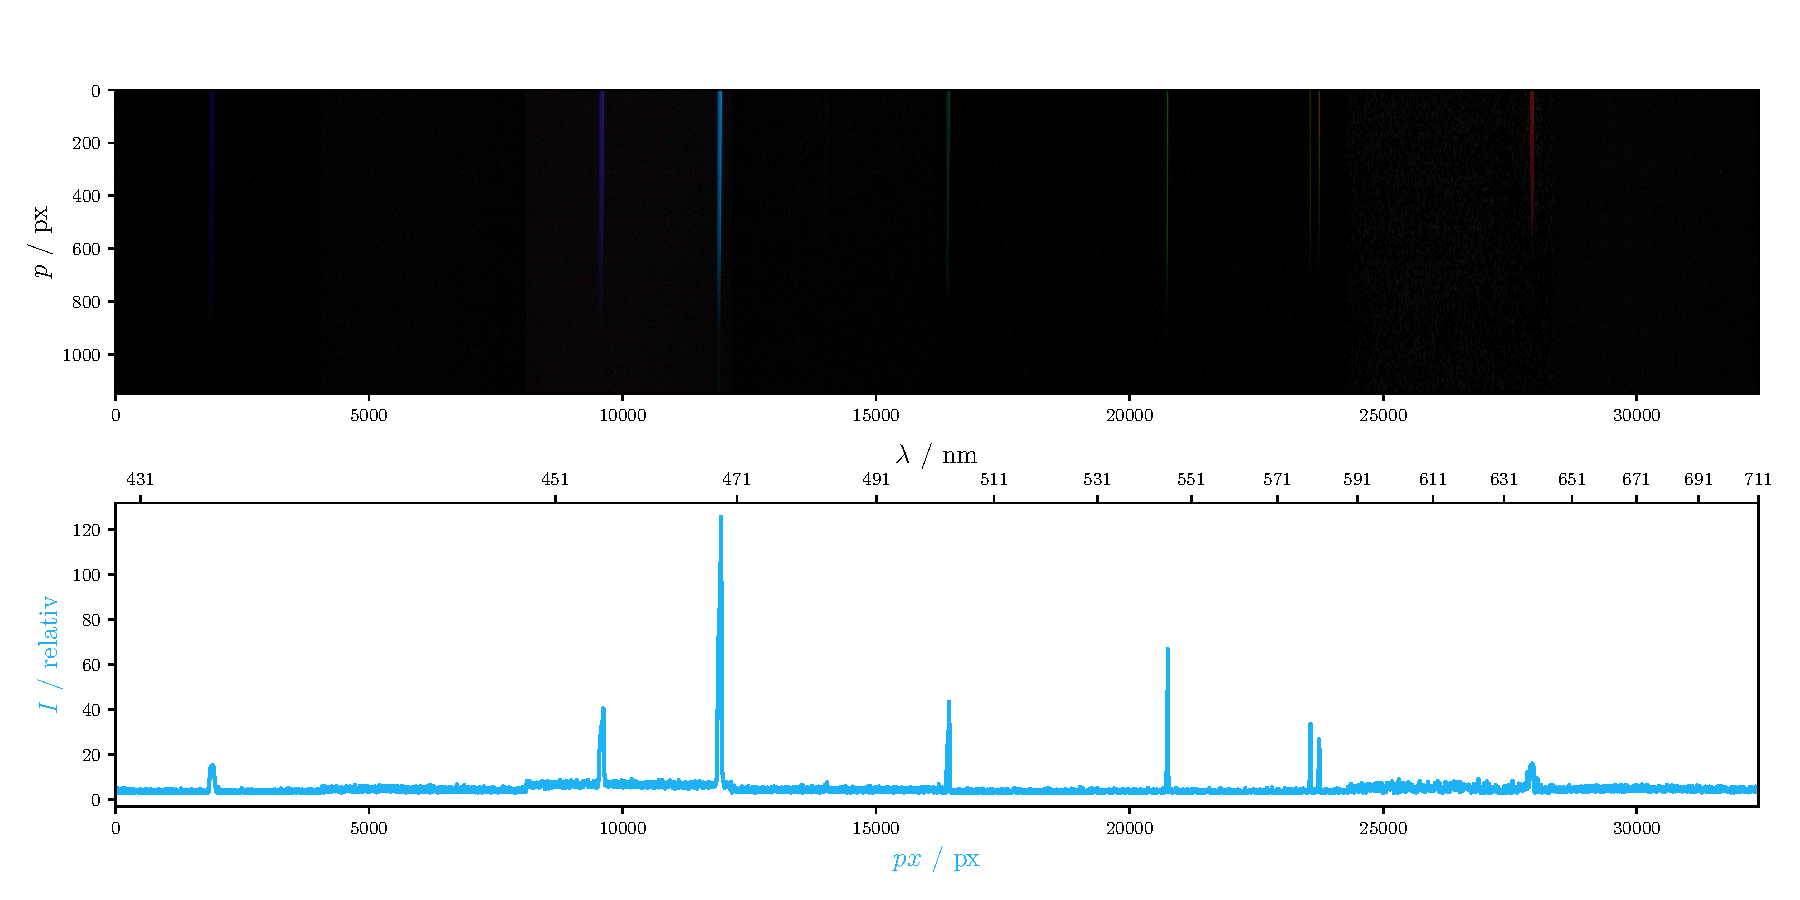
\includegraphics[width=0.95\textwidth]{figures/Hg_plot.pdf}
	\end{center}
	\caption{}\label{fig:prismaHgSpektrum}
\end{figure}

Dieses Spektrum wird verwendet um die Dispersionrelation des Prismas zu finden
und einen Isomorphismus zwischen Pixel und Nanometer erstellen. Unter
Verwendung dieses Isomorphismus wurde den Pixeln in diesen Graphiken auch eine
Wellenlänge zugeordnet. Mehr dazu in \autoref{sec:DispersionPrism}.

Nun wird das Halogenspektrum dargestellt, siehe
\autoref{fig:prismaHaloSpektrum}. 
\begin{figure}[H]
	\begin{center}
		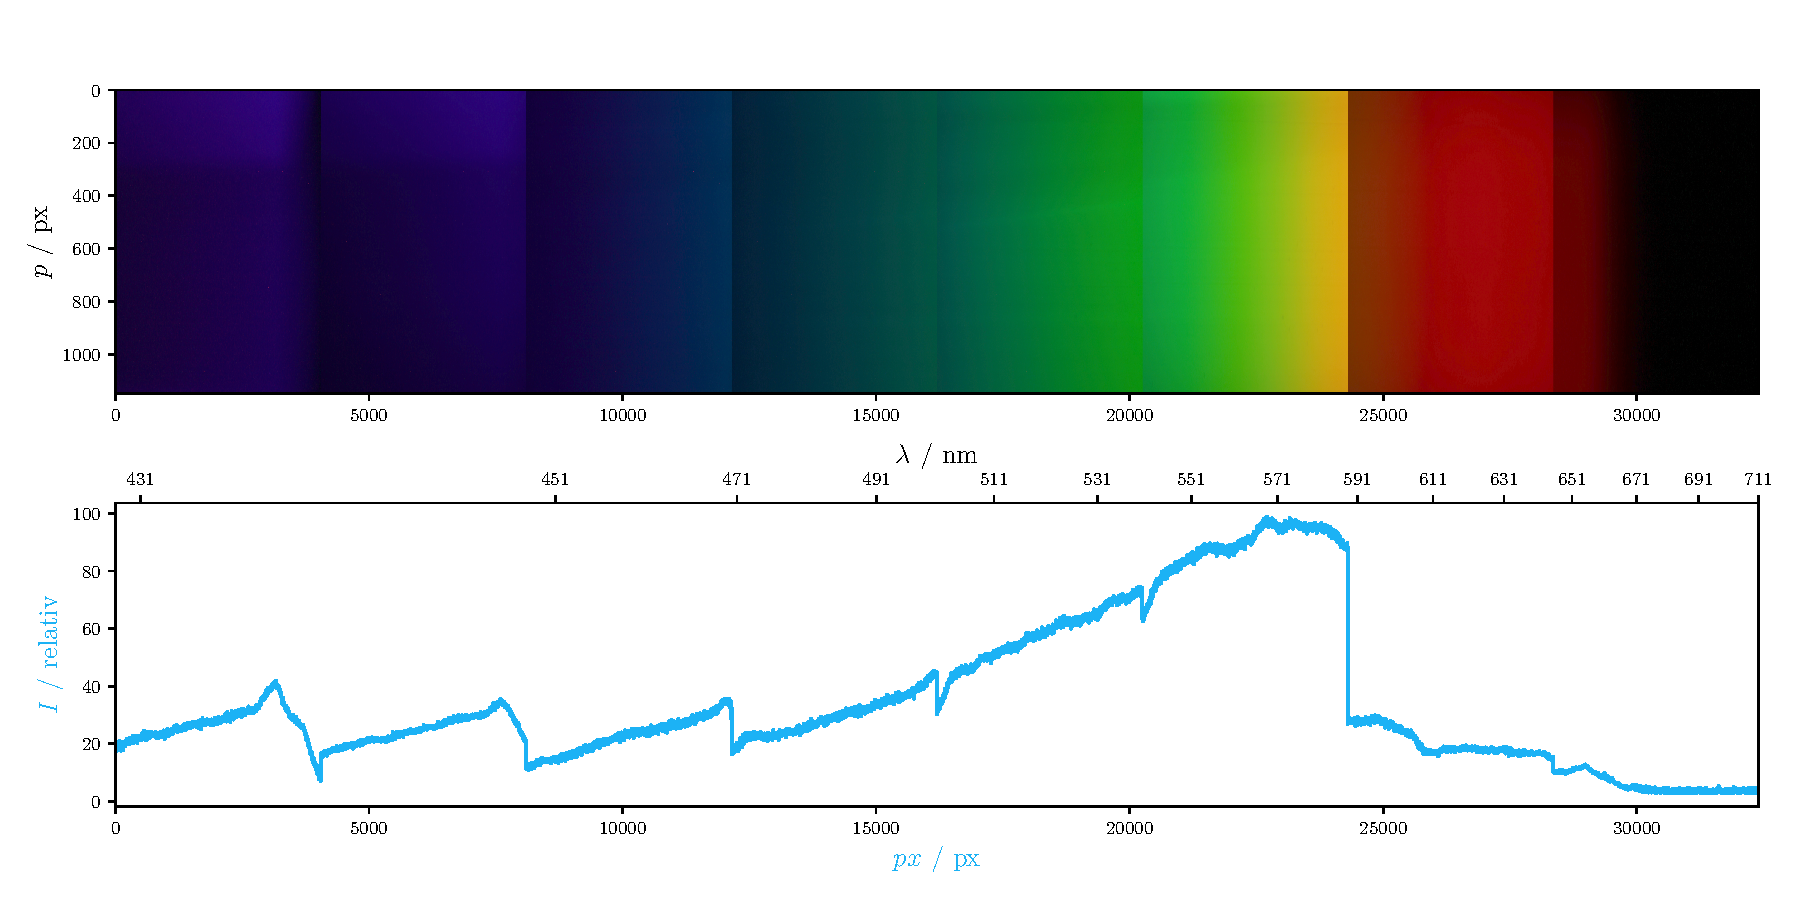
\includegraphics[width=0.95\textwidth]{figures/Halo_plot.pdf}
	\end{center}
	\caption{}\label{fig:prismaHaloSpektrum}
\end{figure}

Zuletzt nun das Spektrum von Iod beleuchtet mit der Halogenlampe, siehe
\autoref{fig:prismaIodSpektrum}.

\begin{figure}[H]
	\begin{center}
		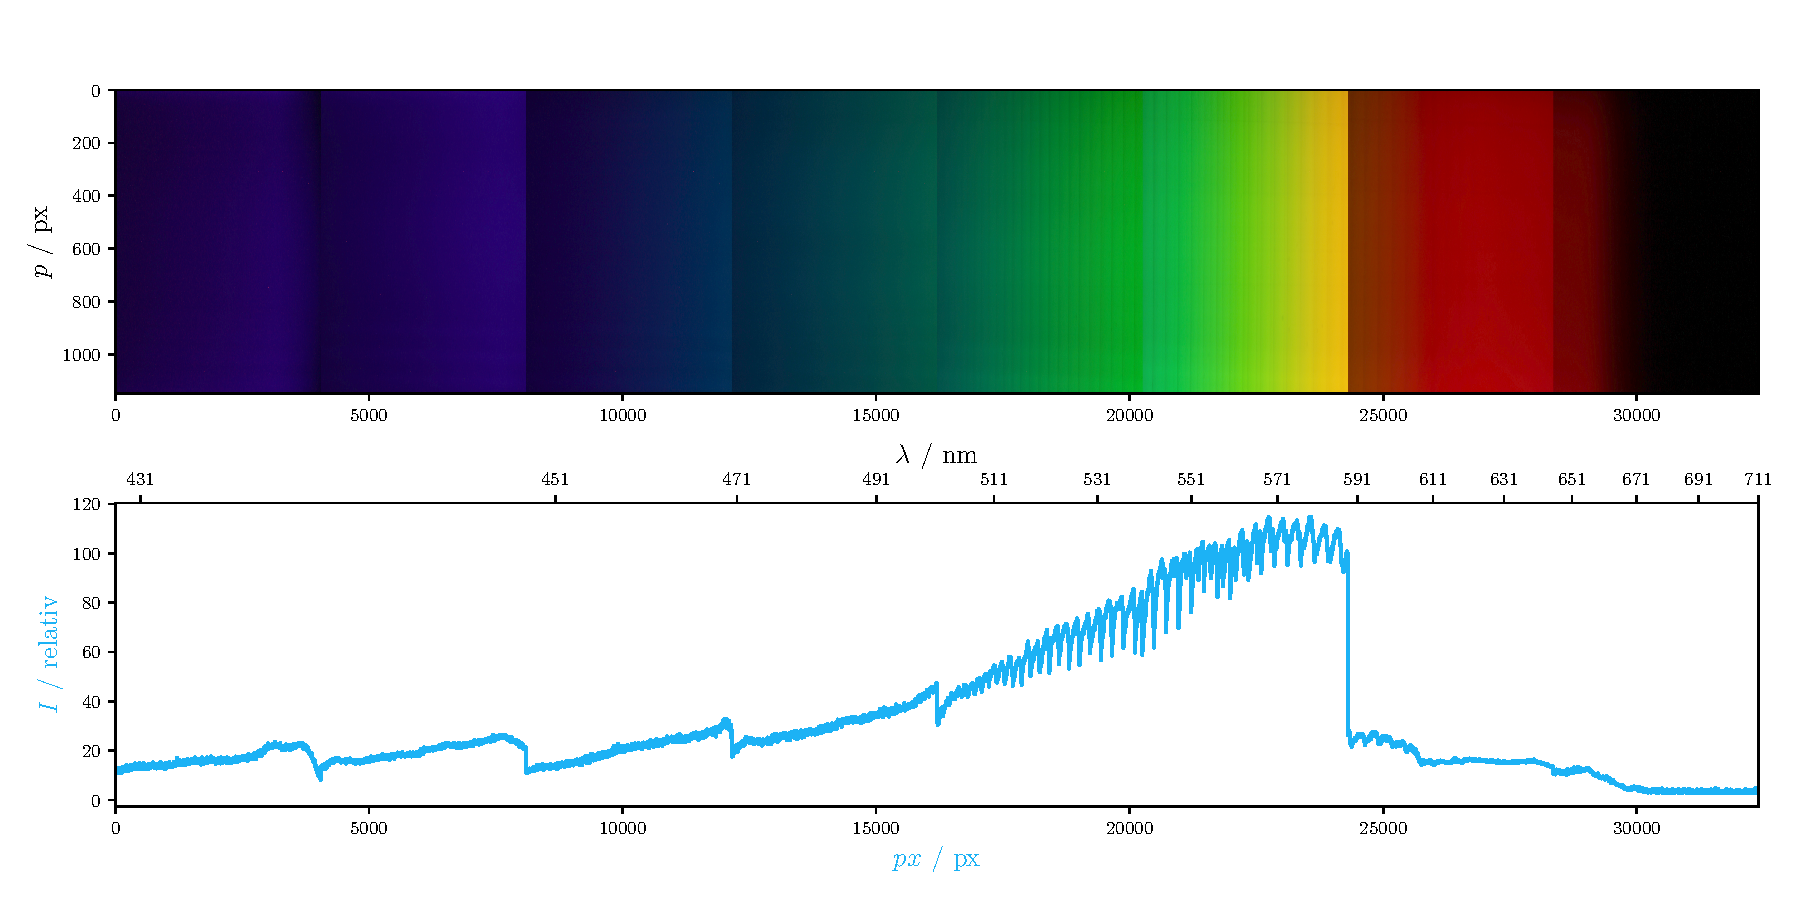
\includegraphics[width=0.95\textwidth]{figures/I_plot.pdf}
	\end{center}
	\caption{}\label{fig:prismaIodSpektrum}
\end{figure}

\subsubsection{Dispersionskurve des Prismenspektrographen}\label{sec:DispersionPrism}

Durch Identifikation der Peaks im Referenzspektrum und der Zuordnung mit den
bekannten Wellenlängen dieser Peaks, aus der Angabe~\cite{}, ist es möglich die
Dispersionskurve mittels eines quadratischen Fit (in Scheitelpunktform $\lambda
	= a (x-b)^2 + c$) zu beschreiben. Da jedoch nur gewisse Wellenlängen der Peaks
bekannt sind und der Cyan Peak bei unserer Messung nicht aufscheint, sind
folgende Wellenlängen und deren zugeordneten Peaks fürs Fitten genommen worden.

\begin{enumerate}
	\item Rot \SI{643.9}{\nano\meter}
	\item Gelb 1 \SI{579.0}{\nano\meter}
	\item Gelb 2 \SI{576.9}{\nano\meter}
	\item Grün \SI{546.0}{\nano\meter}
	\item Türkis \SI{508.5}{\nano\meter}
	\item Blau \SI{467.8}{\nano\meter}
\end{enumerate}

\begin{figure}[H]
	\begin{center}
		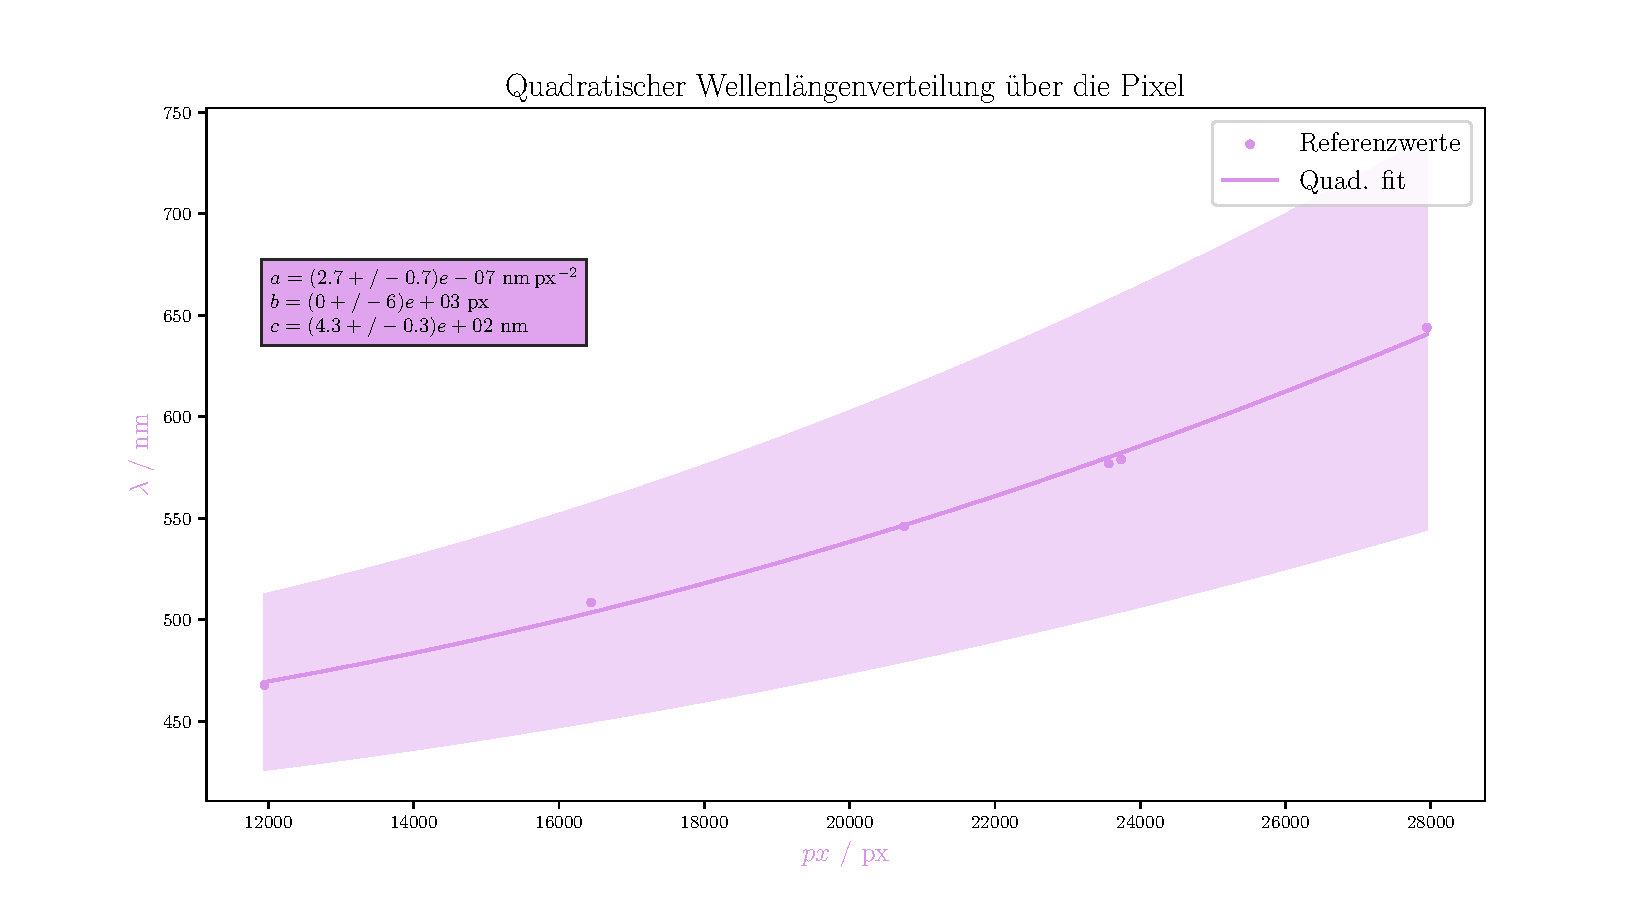
\includegraphics[width=0.95\textwidth]{figures/mappingPxToWaveLength.pdf}
	\end{center}
	\caption{}\label{fig:dispersionkurve}
\end{figure}

Diese gefittet Funktion wird nun, wann auch immer beim Prismenspektrometer von
Pixel zu Nanometer und dessen Inverse wenn Nanometer zu Pixel umgerechnet
werden muss.

\subsection{Gitterspektrometer}

Hier werden nun die Intensität-Spektren der verschiedenen Belichtungen des
Gitterspektrometer dargestellt.

\begin{figure}[H]
	\begin{center}
		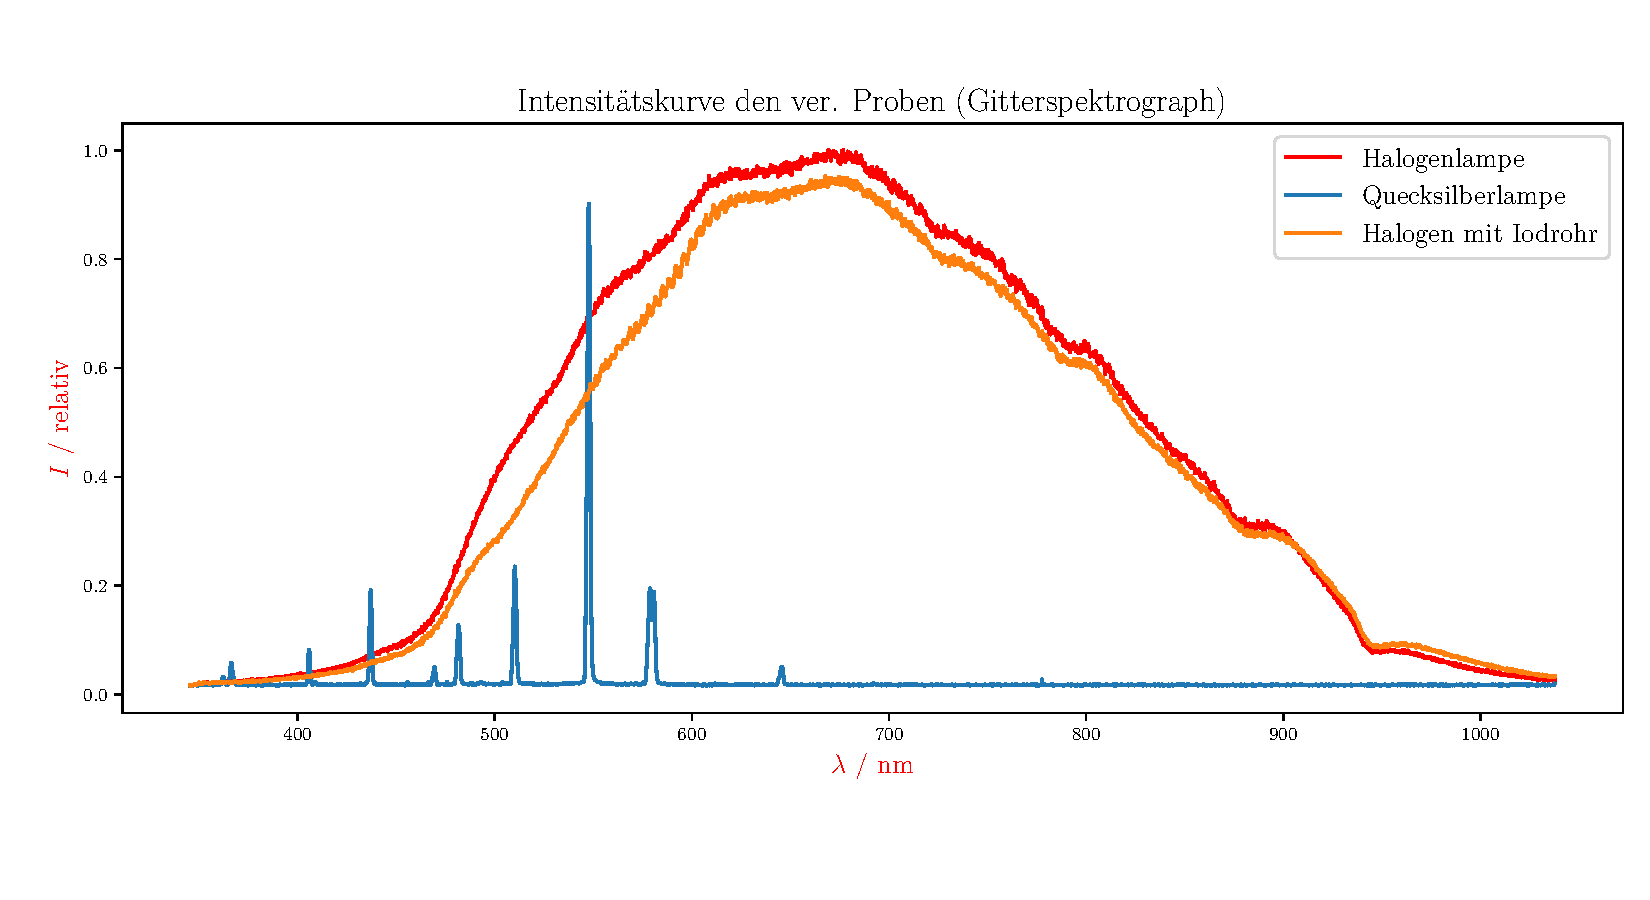
\includegraphics[width=0.95\textwidth]{figures/intensity_spektrum_gitter.pdf}
	\end{center}
	\caption{}\label{fig:spektraGitter}
\end{figure}

\subsubsection{Wellenlänge der Jod-Absorbtionsbandkanten}
Um die Valleys im Absorptionsband von Iod besser finden zu können wird die
Extinktion gebildet indem das Halogenspektrum als Referenzspektrum dient. 

\begin{figure}[H]
	\begin{center}
		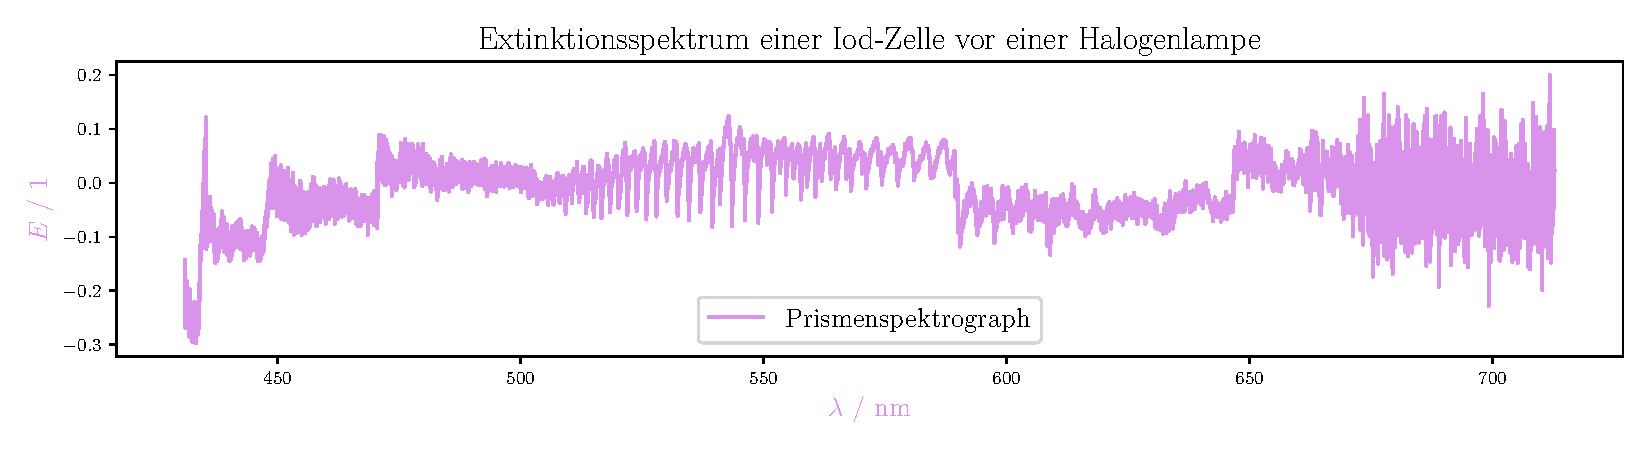
\includegraphics[width=0.95\textwidth]{figures/prism_extinction.pdf}
		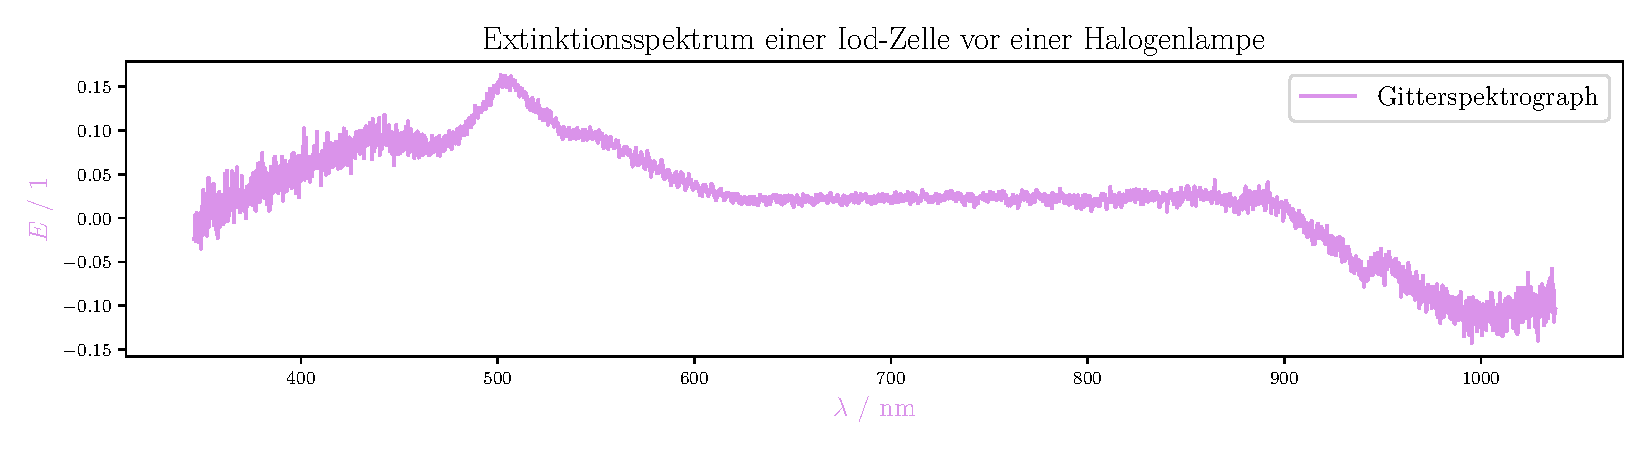
\includegraphics[width=0.95\textwidth]{figures/gitter_extinction.pdf}
	\end{center}
	\caption{}\label{fig:extinktionkurven}
\end{figure}

Zudem wird die Extinktion negiert damit die Valleys zu markante Peaks werden,
welche leicht mittels Vorhanden Peak-Finding-Algorithmen gefunden werden kann.
Dabei wurde sich auf markante Bereich der Extinktionsspektren fokussiert, wo
die Absorption klar ersichtlich sind. Damit ist die einfache Findung und
Bearbeitung der Peaks gewährleistet.

\begin{figure}[H]
	\begin{center}
		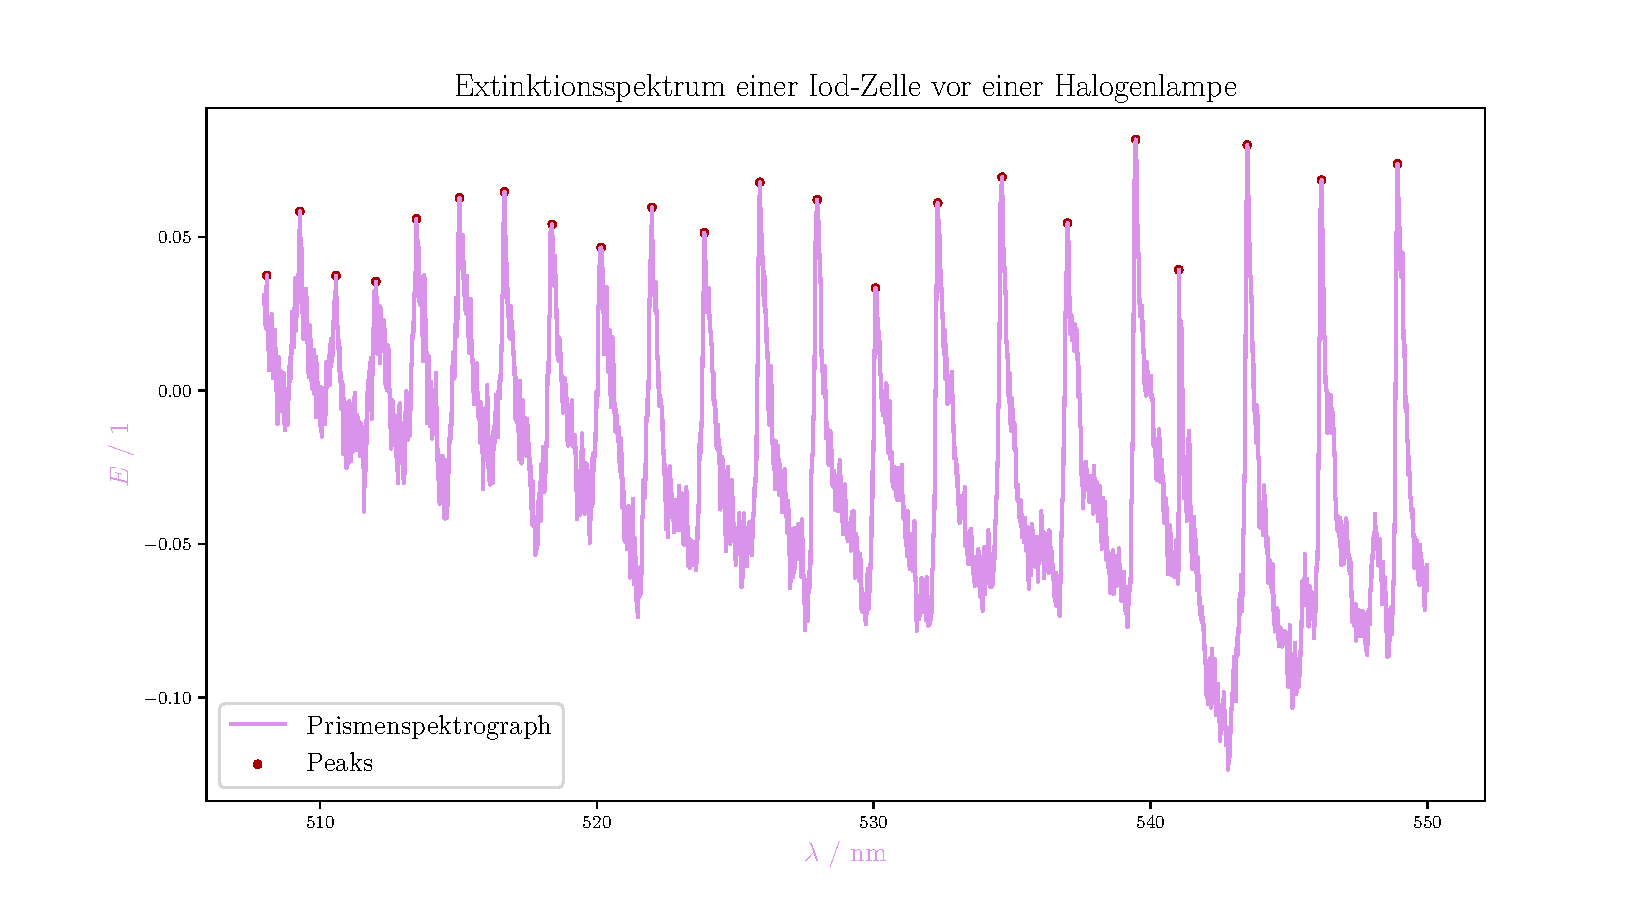
\includegraphics[width=0.95\textwidth]{figures/prism_ausschnitt_extinction.pdf}
		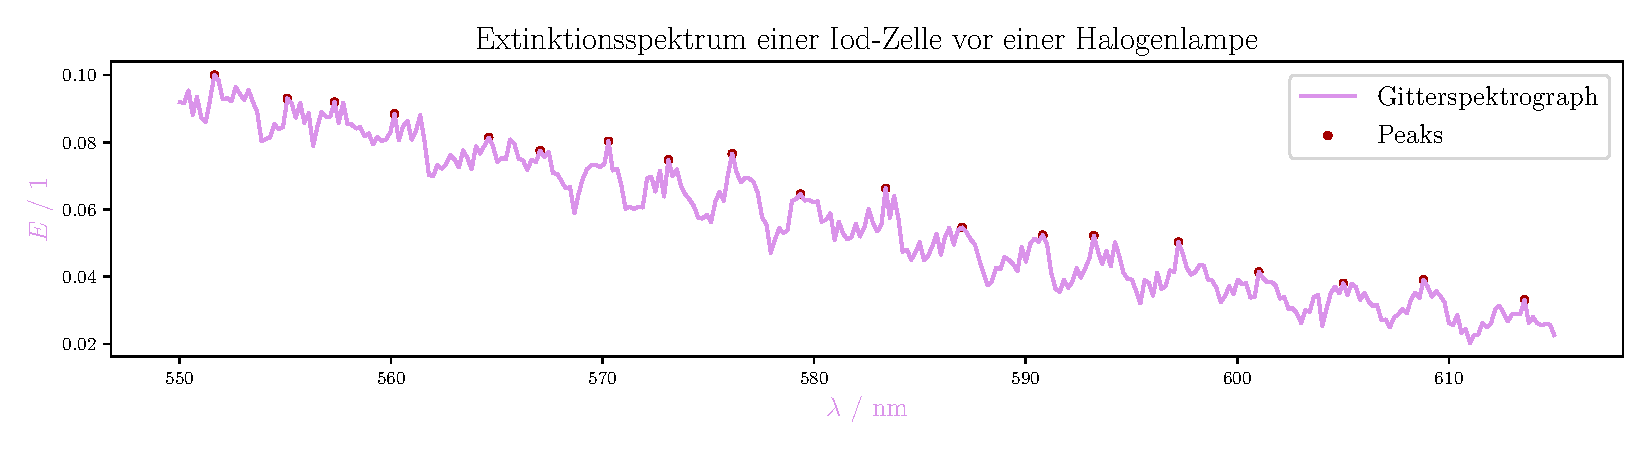
\includegraphics[width=0.95\textwidth]{figures/gitter_ausschnitt_extinction.pdf}
	\end{center}
	\caption{}\label{fig:ausschnittPeaks}
\end{figure}

Da diesen Peaks gleich eine Wellenlänge zu geordnet wird kann die Wellenlänge
der Bandlücke abgelesen werden.

Die Wellenlängen der Peaks lassen nochmals mittels eines quadratischen Fits (in
Scheitelpunktform $\nu = a (x-b)^2 + c$) beschreiben und finden dadurch einen
Isomorphismus zwischen den Indexes und deren Wellenzahlen $\nu$.

\begin{figure}[H]
	\begin{center}
		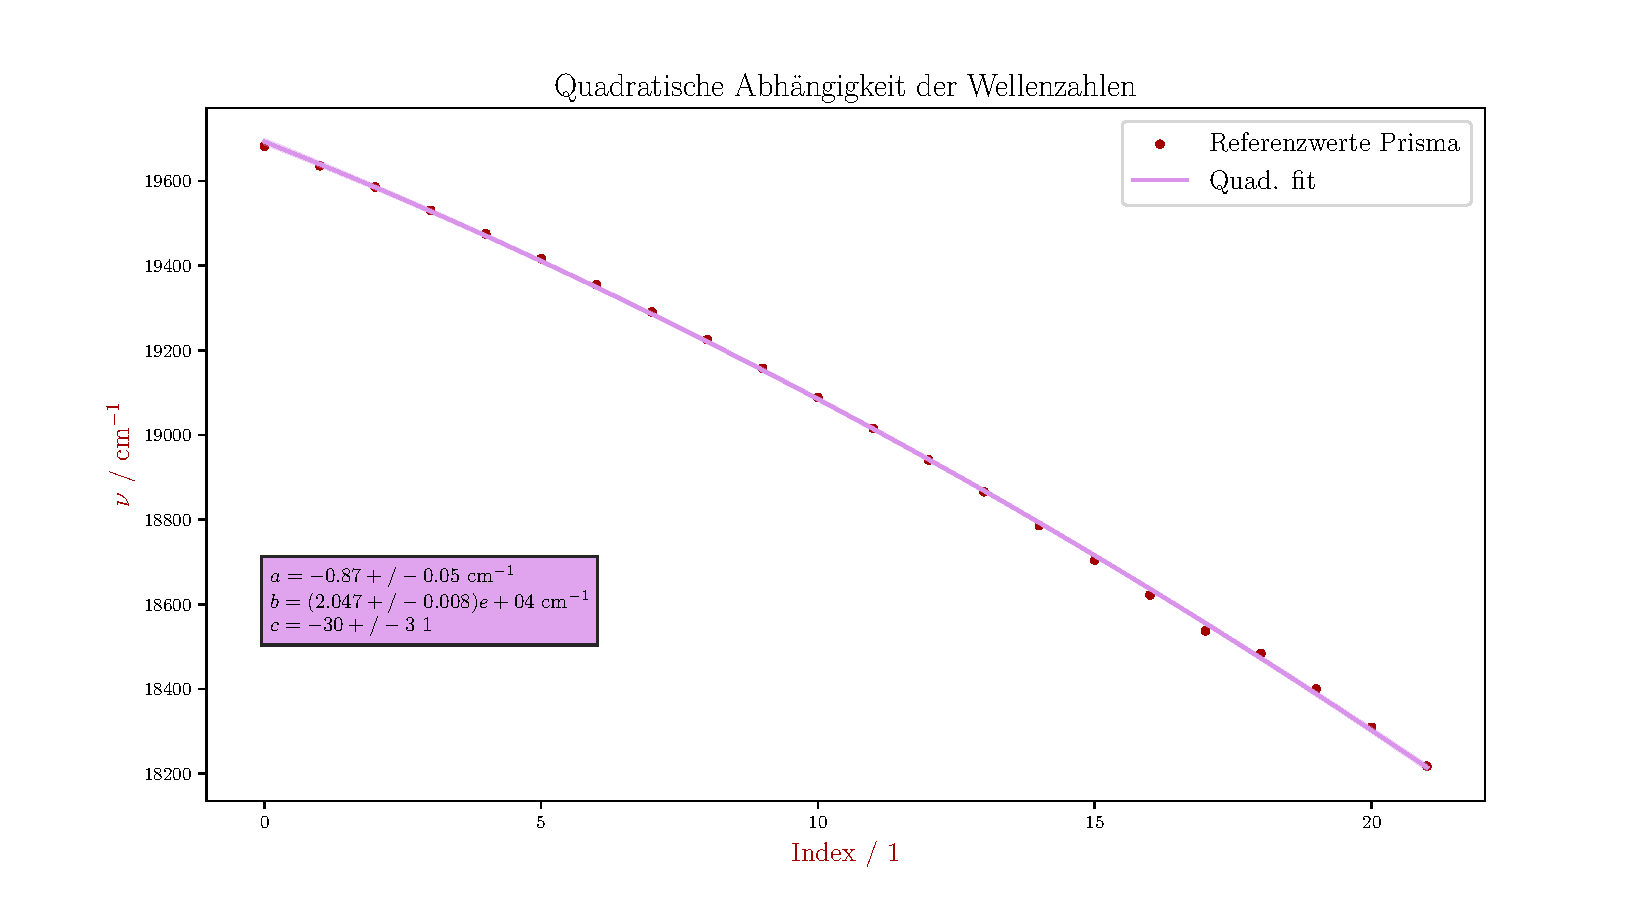
\includegraphics[width=0.95\textwidth]{figures/waveNumberFitPrisma.pdf}
		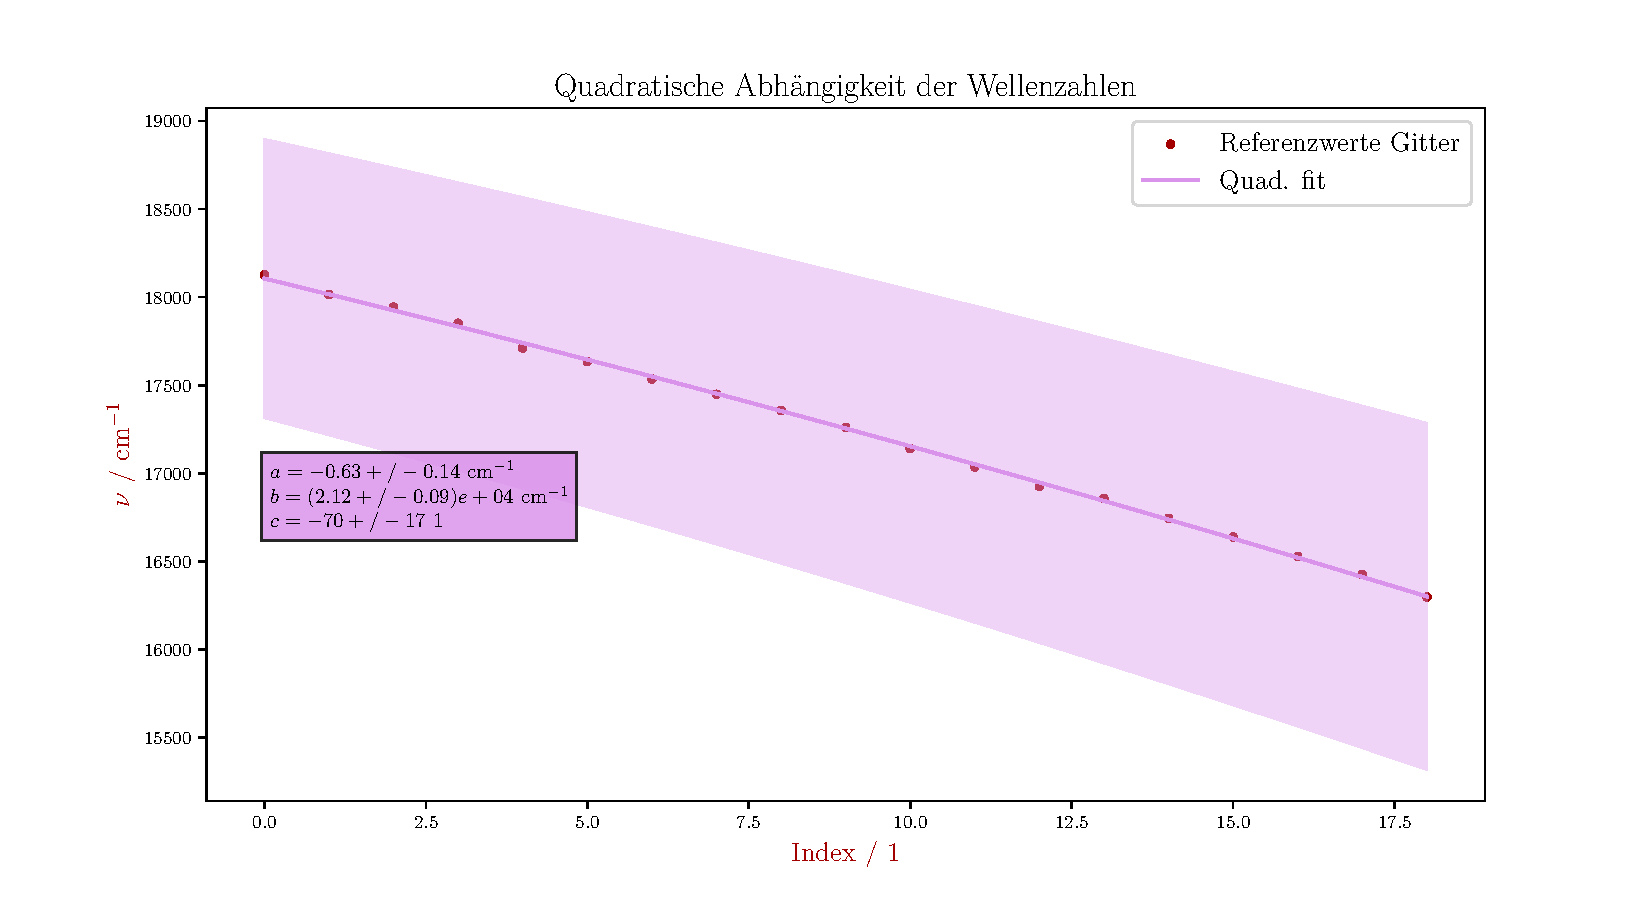
\includegraphics[width=0.95\textwidth]{figures/waveNumberFitGitter.pdf}
	\end{center}
	\caption{}\label{fig:wellenZahlenFit}

\end{figure}

Die Differenzen der Wellenzahlen können auf Grund der quadratischen Natur der
$\nu$ als lineare Funktion modelliert und gefittet werden.

\begin{figure}[H]
	\begin{center}
		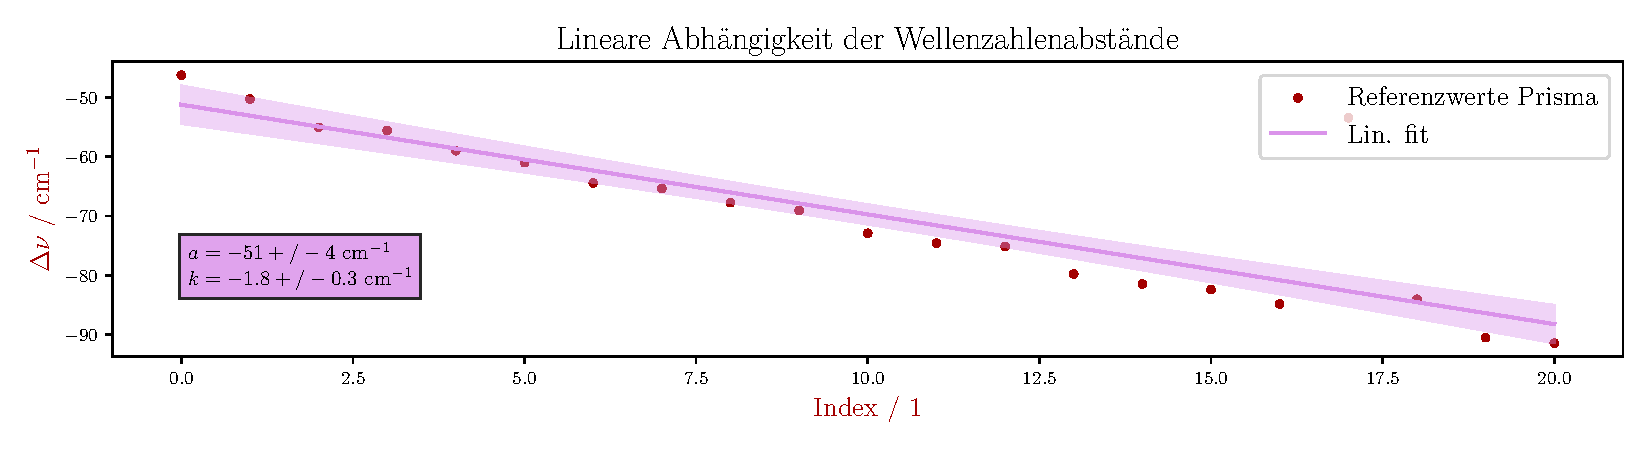
\includegraphics[width=0.95\textwidth]{figures/waveNumberDeltasFitPrisma.pdf}
		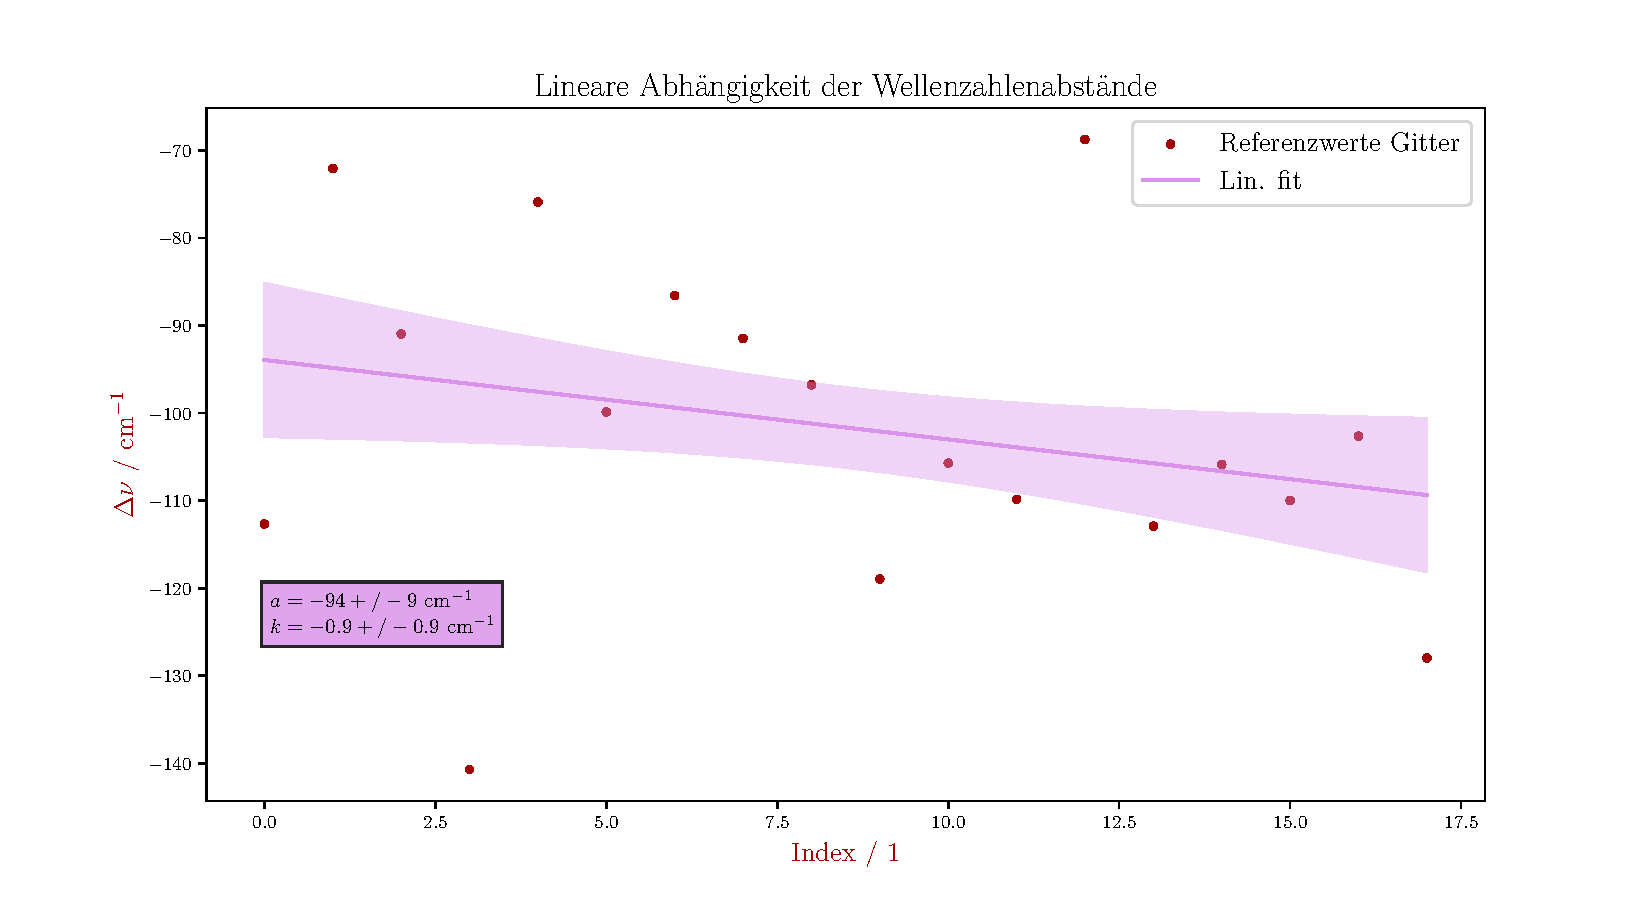
\includegraphics[width=0.95\textwidth]{figures/waveNumberDeltasFitGitter.pdf}
	\end{center}
	\caption{}\label{fig:wellenZahlenDeltaFit}

\end{figure}

Diese Funktion modelliert die Steigung des Isomorphismus und erlaubt uns den
Extreme Wert für die Wellenzahl zu finden.

\subsubsection{Dissoziationsenergie des Jodmoleküls}
Aufgrund der größeren Unsicherheit des linearen Fits beim Gitterspektrometer,
in \autoref{fig:wellenZahlenDeltaFit}, wird nur die Auswertung für den
Prismenspektrometer gemacht.

Indem in die invertierte lineare Funktion vom Fit 0 eingesetzt wird kann der
Index gefunden werden für den die Wellenzahl im Isomorphismus maximiert wird
(siehe Vorzeichen der quadratischen Funktion).

Die maximierte Wellenzahl ist:
\begin{equation}
	\nu = \SI{2.047(9)e6}{\per\cm}
\end{equation}

Mittels der Strahlungsenergieformel ist die Scheitelpunktsenergie zu berechnen:
\begin{equation}
	E_s = h c \nu = \SI{4.066(17)e-19}{\joule} = \SI{2.538(11)}{\electronvolt}
\end{equation}

Zieht man Schlussendlich die Anregungsenergie
$E_A=\SI{0.970(5)}{\electronvolt}$ von der Scheitelpunktsenergie ab erhält man
die Dissoziationsenergie:

\begin{equation}
	E_\text{Diss} = E_s - E_A = \SI{1.568(12)}{\electronvolt}
\end{equation}

\subsection{Auflösevermögen}

% TODO

\section{Diskussion}\label{sec:disk}

\subsection{Prismenspektrograph}

Allgemein ist die Benutzung des Prismenspektrographen sehr aufwändig, weil die
Justierung der Linsen und Prismen sehr viel Zeit in Anspruch nimmt. Auch ist
die Aufnahme des Spektrums, welches sich aus mehreren Einzelbildern
zusammensetzt, klar zeitintensiver.

Beim Betrachten des Spektrums aus \autoref{fig:prismaHaloSpektrum} wird klar
ersichtlich, dass die Linien durch diverse Abbildungsfehler eine leichte
Krümmung aufweisen. Besonders stark ist dieser Effekt bei den niedrigeren
Wellenlängen, was sich durch die höhere Energie erklären lässt. Für die
Auswertung wurde dadurch nur ein schmaler Bereich aus der Mitte genommen, um
die Werte nicht durch diese Krümmung zu verfälschen. Die schärfe der Kamera
wurde auf den gelbe Doppellinie bei \SI{579.0}{\nano\meter} und
\SI{576.9}{\nano\meter} fokussiert, da diese besonders signifikant für die
Lichtquelle ist.

\subsection{Gitterspektrograph}

Der Vorteil des Gitterspektrographen liegt vor allem in der einfachen
Handhabung. So muss dieser nur angeschlossen werden und liefert sofort einen
Intensitätsverlauf. Jedoch wird kein Spektrum erzeugt. Auch ist darauf zu
achten, dass die erzeugt Grafik nicht übersättigt ist, was zu einem Fehler
führen würde.

Im Bezug auf die Genauigkeit des Gitterspektrographen sei angemerkt, dass
dessen letzte Kalibrierung im Jahr 2008 stattgefunden hat, was darauf schließen
lässt, dass eine erneute Kalibrierung die Genauigkeit verbessern könnte.

\subsection{Auflösevermögen}
Die erhaltenen Werte der Auflösevermögen sind in folgender
\autoref{tab:vergleich_auflosung} gegenübergestellt.

%todo vergleich der Werte
Ein Vergleich dieser Werte zeigt klar, dass der Prismenspektrograph eine
deutlich höhere Auflösung hat. Dies wird auch bei der qualitativen Betrachtung
der entsprechenden Bilder sichtbar.

\subsection{Dissoziationsenergie des Jodmoleküls}

Die erhaltenen Werte für die Dissoziationsenergie sind in folgender
\autoref{tab:vergleich_disotiation} dem Literaturwert gegenübergestellt.

%todo vergleich der Werte
Der Literaturwert ist also in beiden Fehlerintervallen enthalten. Der erhaltene
Wert des Prismenspektrographen liegt jedoch deutlich näher am Literaturwert.
Auch ist dessen Unsicherheit kleiner.

\section{Zusammenfassung}\label{sec:zs}
Zunächst lässt sich feststellen, dass die Handhabung des Gitterspektrographen
deutlich einfacher und vor allem schneller geht. Die erhaltenen Ergebnisse des
Prismenspektrographen sind jedoch genauer am Literaturwert und haben auch eine
geringere Unsicherheit. Weiters liegt auch eine bessere Auflösung vor. Wodurch
sich der Zeitaufwand insgesamt lohnt. Es sei jedoch auch angemerkt dass sich
die Untersuchung von Lichtquellen durch den Prismenspektrographen nur für
Lichtquellen eignet, die leicht zum Spektrographen gebracht werden können, da
dieser aufgrund seiner Größe und des Justierungsaufwands nur sehr schwer bewegt
werden kann.

\subsection{Spektren}

Im Rahmen dieses Praktikums wurden die Spektren einer Hg-Lampe, einer
Halogenlampe und einer Jodprobe, sowohl mit einem Prismenspektrographen als
auch mit einem Gitterspektrographen bestimmt. Die erhaltenen Spektren sind in
den \autoref{fig:prismaHgSpektrum} \autoref{fig:prismaHaloSpektrum}
\autoref{fig:prismaIodSpektrum} und \autoref{fig:spektraGitter} ersichtlich.

\subsection{Auflösevermögen}

Die erhaltenen Werte für die Auflösevermögen sind in folgender
\autoref{tab:zs_auflosevermogen} ersichtlich.
%todo tab

\subsection{Wellenlänge der Jod-Absorbtionsbandkanten}

%todo 

\subsection{Dissoziationsenergie des Jodmoleküls}

Der erhaltene Werte für die Dissoziationsenergie ist $E_\text{Diss} =
	\SI{1.568(12)}{\electronvolt}$ und der Literaturwert ist
$E_{\text{Diss}_\text{lit}} = \SI{1.57}{\electronvolt}$

\newpage

\section{Appendix}\label{sec:Appendix}
\subsection{Code}\label{sec:code}
\lstinputlisting[language=Python,caption=For Merging the recorded images and determination of the dispersion relation. The resoltion power of the prism was also determined.]{./analysis/imageprep.py}
\lstinputlisting[language=Python,caption=The wavelength extraction of the band eges in the Iodine absorptions spectrum and calculation of the dissociation energy of iodine molecule in ground state.]{./analysis/extinction.py}

% \printbibliography
\listoffigures
\listoftables
\end{document}
